\chapter{Results and discussion}\label{chap:Results&Disc}
\section{PFCA sorption}
\subsection{Biochar-water sorption isotherms}
\cref{fig:sorption_isotherms} shows the sorption isotherms for PFPeA, PFHxA, PFHpA, PFOA, PFNA and PFDA on CWC, ULS and DSL biochars. The points generated from the batch tests were fitted using the Freundlich model (\cref{eq:FreundlichLinear}). For all compounds, the sorption isotherm for ULS was visibly higher than DSL, followed by CWC. The Freundlich sorption coefficients ($\log~K_F$), linearity coefficients ($n_F$), and correlation coefficients ($r^2$) are presented in \cref{tab:summary_stats_single}. 

Based on measurements made in this study, sorption is strongest for the two sludge chars. This was unexpected. Possible mechanisms that could account for these findings will be discussed in this chapter. Research on the sorption of PFAS to sewage sludge is relatively new. To the best of this author's knowledge, there is no current literature available that demonstrates partitioning coefficients for PFAS to other sewage sludge biochars that are comparable with the ones found in this study. However, comparisons can be made between the $\log~K_F$s found in this thesis, and commercially-produced activated carbons (AC) reported in previous studies. Sorption coefficients in this study (5.12-5.73) are equivalent to, or higher than, values for $\log~K_F$ of PFOA to AC found in other literature: 5.60 \citep{Kupryianchyk2016b}, 4.45 \citep{hansen2010sorption}, and 4.74-5.42 \citep{silvani2019can}. 

The slope ($n_F$) of the linear regression equation obtained from the $\log~C_w$ versus $\log~C_s$ concentration points, represents how linear the isotherm is within the concentration intervals achieved. All BC single isotherms have $n_F<1$. This indicates that the concentration interval achieved shows some degree of attenuation (\cref{tab:summary_stats_single}. This is consistent with other studies where sorption to biochar has $n_F$-values, typically, around 0.3-0.7 \citep{Cornelissen2005}. The slopes that have $n_F>1$ (PFHxA-DSL: n=1.11 and PFHpA-ULS: 1.08) are not statistically higher than 1 (standard error $\pm$ 0.11 for both). For the short-chain compounds (PFPeA and PFHxA), correlations were poor. Results for these insignificant isotherms have not been reported. 

\begin{figure}[tb]
    \centering
    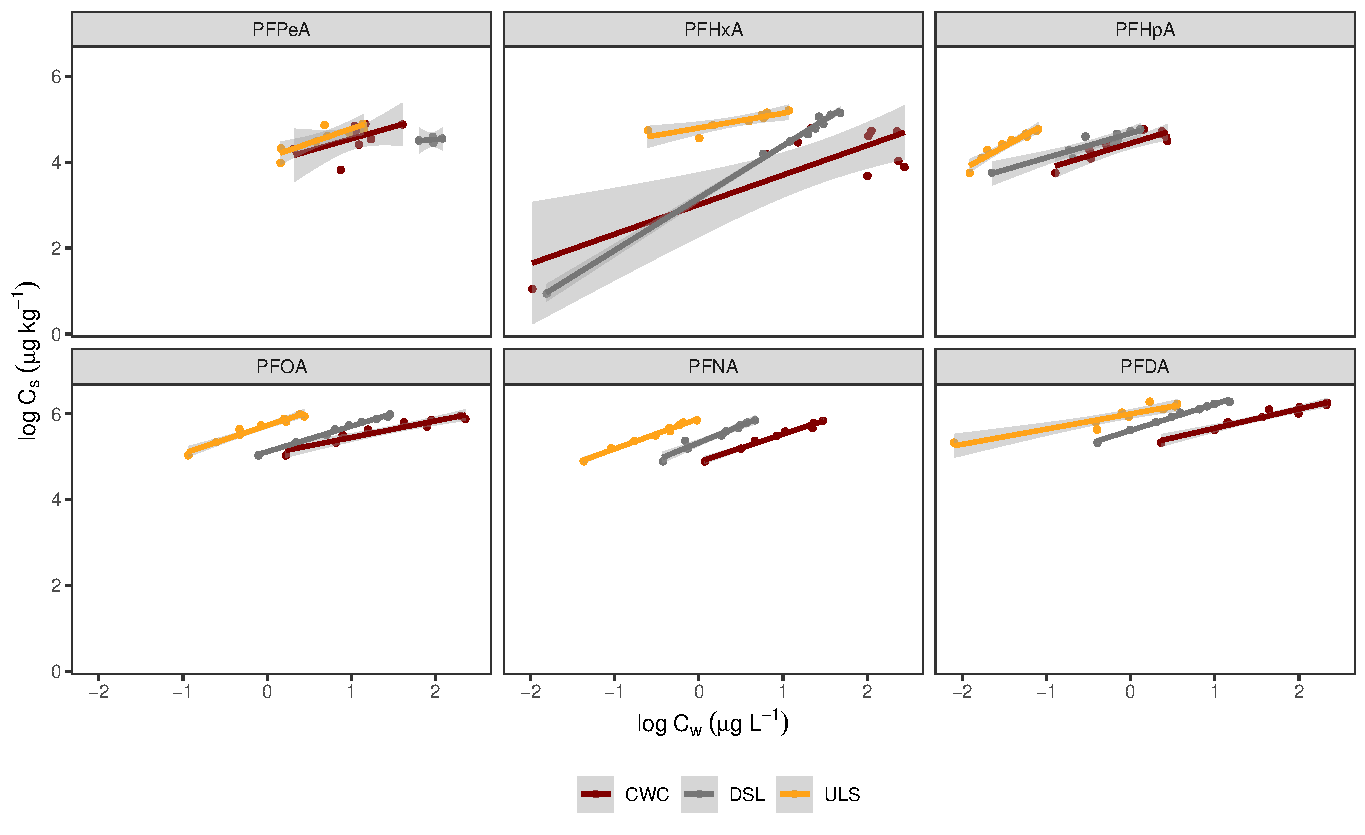
\includegraphics[width=\textwidth]{R/figs/Sorption_isotherms_single_BC.pdf}
    \caption{Freundlich sorption isotherms for PFPeA, PFHxA, PFHpA, PFOA, PFNA and PFDA in batch tests with three different biochars. Lines are obtained by linear regression.}
    \label{fig:sorption_isotherms}
\end{figure}

\begin{table}
\caption{Freundlich sorption coefficients and linear regression statistics for the BC-single isotherms in CWC, ULS and DSL (n=9). The error is presented as standard error. All $K_F$ data are in units of $\mathrm{(\mu g/kg)/(\mu g/L)^{n_F}}$.}
\centering
\adjustbox{max width=\textwidth}{%
\begin{threeparttable}
\label{tab:summary_stats_single}
\begin{tabular}{lllllllllllll} \toprule
PFCA & \multicolumn{4}{c}{ULS} & \multicolumn{4}{c}{DSL} & \multicolumn{4}{c}{CWC} \\ \cmidrule(l){2-5} \cmidrule(l){6-9} \cmidrule(l){10-13}
 & $\log~K_{F,BC}$ & $n_{F,BC}$ & $r^2$ & $p$ & $\log~K_{F,BC}$ & $n_{F,BC}$ & $r^2$ & $p$ & $\log~K_{F,BC}$ & $n_{F,BC}$ & $r^2$ & $p$ \\ \midrule
PFPeA & 4.10 ± 0.13 & 0.67 ± 0.16 & 0.74 & ** &  &  &  & $>$0.05 &  &  &  & $>$0.05 \\
PFHxA & 4.80 ± 0.06 & 0.34 ± 0.09 & 0.72 & ** & 3.30 ± 0.15 & 1.11 ± 0.11 & 0.93 & *** &  &  & & $>$0.05 \\
PFHpA & 5.98 ± 0.17 & 1.08 ± 0.11 & 0.93 & *** & 4.67 ± 0.06 & 0.57 ± 0.09 & 0.86 & *** & 4.44 ± 0.05 & 0.59 ± 0.11 & 0.80 & ** \\
PFOA & 5.73 ± 0.02 & 0.65 ± 0.05 & 0.95 & *** & 5.12 ± 0.02 & 0.60 ± 0.02 & 0.99 & *** & 5.06 ± 0.08 & 0.39 ± 0.05 & 0.90 & *** \\
PFNA & 5.89 ± 0.02 & 0.71 ± 0.03 & 0.99 & *** & 5.33 ± 0.03 & 0.80 ± 0.07 & 0.94 & *** & 4.88 ± 0.04 & 0.65 ± 0.04 & 0.98 & *** \\
PFDA & 6.00 ± 0.04 & 0.35 ± 0.05 & 0.86 & *** & 5.61 ± 0.02 & 0.61 ± 0.02 & 0.99 & *** & 5.22 ± 0.07 & 0.45 ± 0.04 & 0.94 & *** \\ \bottomrule
\end{tabular}
\begin{tablenotes}
\item Significance codes: *** $<$ 0.001, ** $<$ 0.01
\item Insignificant regressions (p $<$ 0.05) have been removed
\end{tablenotes}
\end{threeparttable}}
\end{table}

\subsection{Effects of PFCA physicochemical properties on sorption}
\begin{landscape}


\begin{figure}[tb]
    \centering
    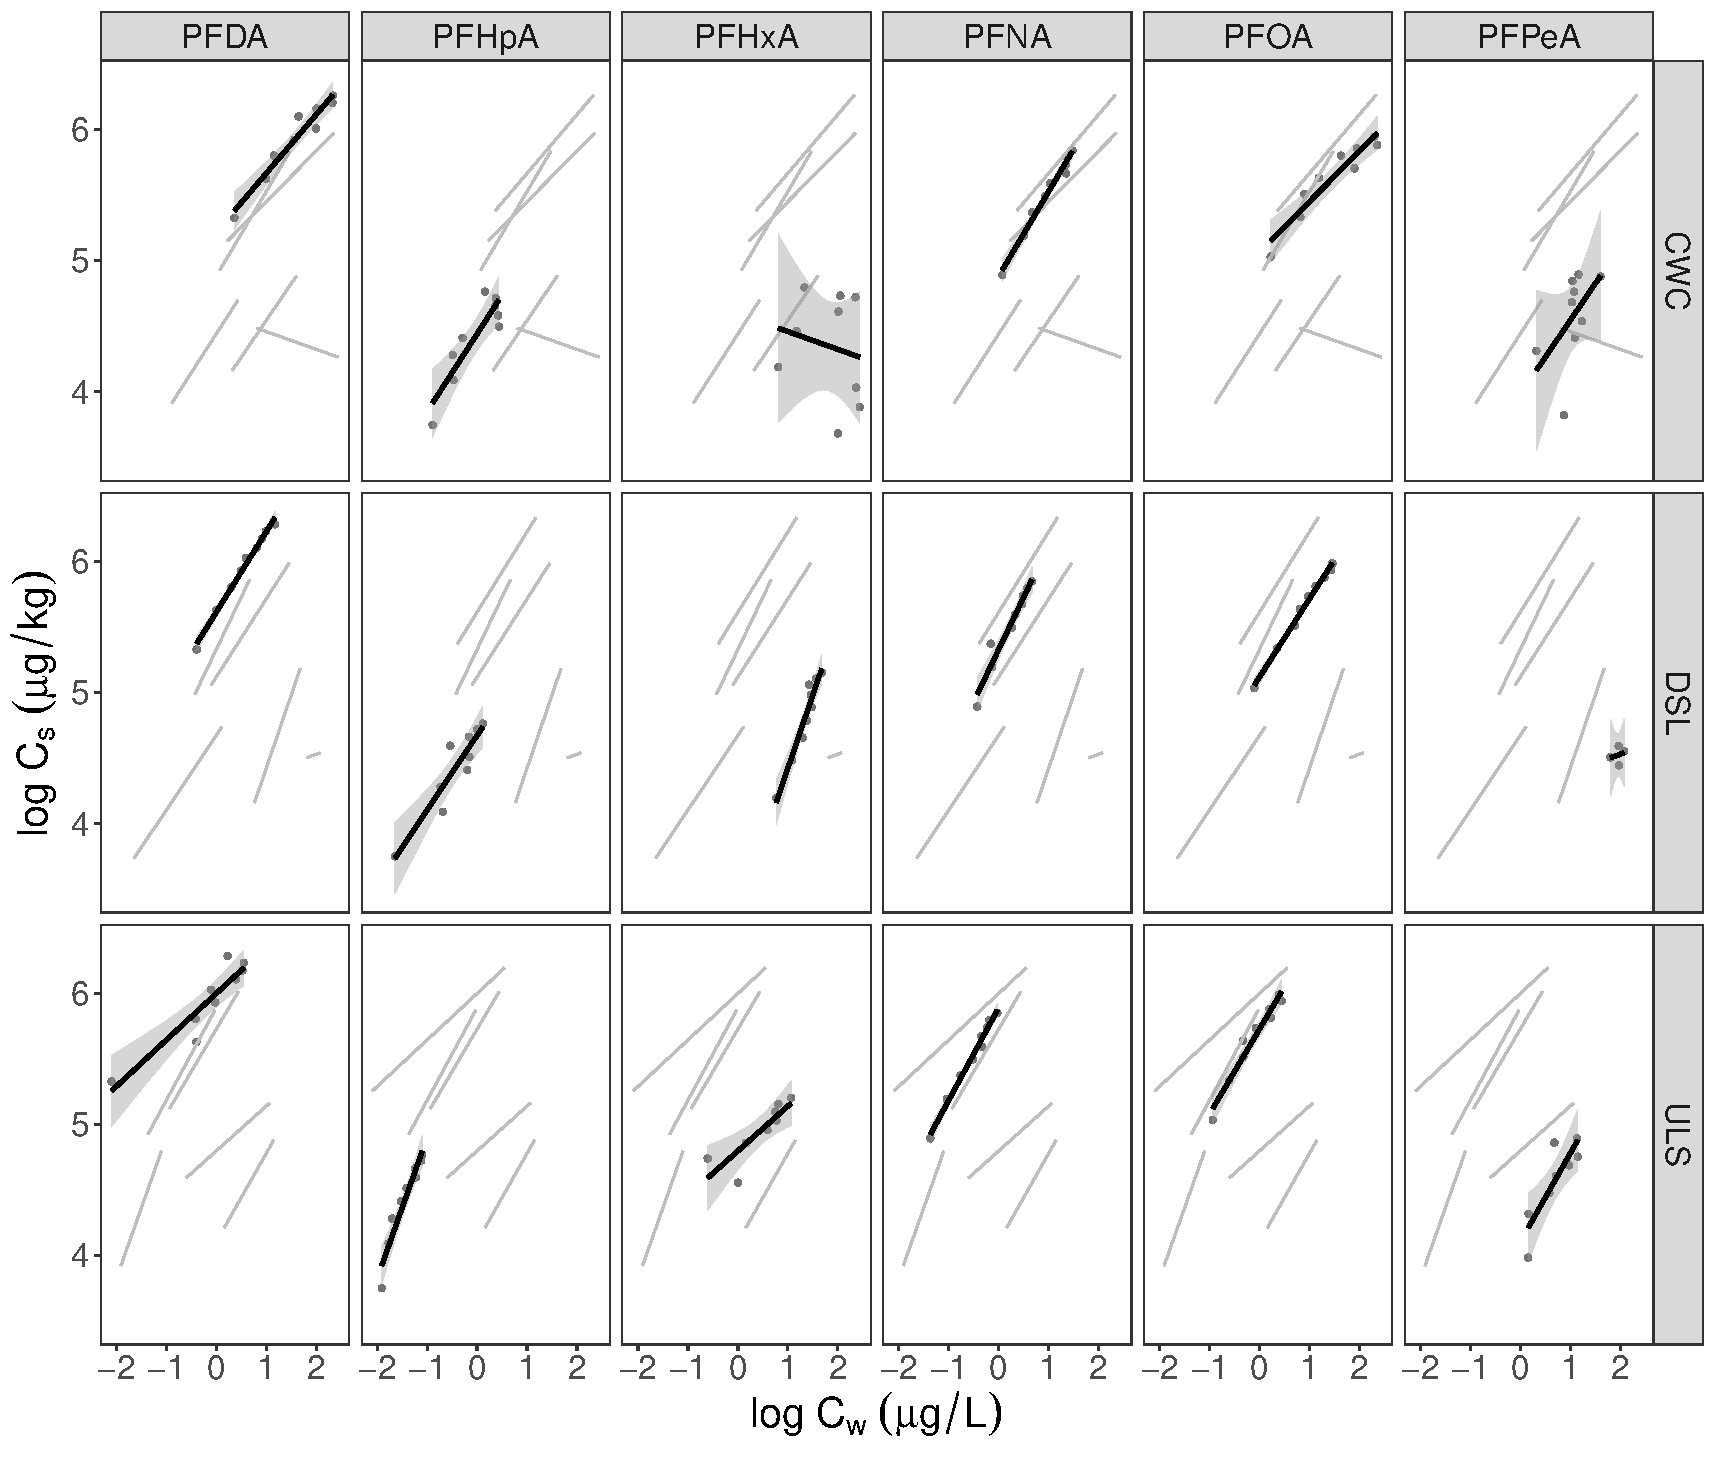
\includegraphics[height=0.8\textheight]{R/figs/BC_facet_isotherm.pdf}
    \caption{Single-compound Freundlich sorption isotherms for PFPeA, PFHxA, PFHpA, PFOA, PFNA and PFDA. Lines are obtained by linear regression. For comparison across chain length, the shaded gray lines are the isotherms from the other compounds with the same sorbent.}
    \label{fig:sorption_isotherms_all}
\end{figure}

\end{landscape} 
\subsubsection{Effects of PFCA chain length}
\Cref{fig:sorption_isotherms_all} shows sorption isotherms for the single-compound batch tests for CWC, ULS and DSL. The Freundlich coefficients ($\log~K_F$) reported are in units of $\mathrm{(\mu g/kg)/(\mu g/L)^{n_F}}$. Sorption to ULS increased in the order: PFPeA (CF4) $<$ PFHxA (CF5) $<$ PFOA (CF7) $<$ PFHpA (CF6) $<$ PFNA (CF8) $<$ PFDA (CF9) where $\log~K_F$ ranged from 4.10$\pm$0.13 to 6.00$\pm$0.04 . Sorption to DSL increased in the order: PFHxA (CF5) $<$ $<$ PFHpA (CF6) $<$ PFOA (CF7) $<$ PFNA (CF8) $<$ PFDA (CF9) where $\log~K_F$ ranged from 3.30$\pm$0.15 to 5.61$\pm$0.02. Sorption to CWC increased in the order: PFPeA (CF4) $<$ PFHpA (CF6) $<$ PFHxA (CF5) $<$ PFNA (CF8) $<$ PFOA (CF7) $<$ PFDA (CF9), where $\log~K_F$ ranged from $\log~K_F$ 3.98$\pm$0.36 to 5.22$\pm$0.07. Insignificant ($p>0.05$) isotherms have not been reported. Poor correlations for the isotherm regressions were achieved for the short-chain PFCAs (PFPeA, PFHxA, and PFHpA) when sorption isotherms were derived. This can be attributed to poor sorption affinity to biochar. All Freundlich coefficients are listed in \cref{tab:summary_stats_single}. 

The sorption of PFAS increased with greater fluorinated chain length. A statistically significant relationship between $\log~K_F$ and CF\textsubscript{2} chain length was found for all three biochars (p$<$0.05) to PFOA, PFNA, and PFDA (\cref{fig:chainlength}) in accordance with previous studies \citep{Sorengard2019, fabregat2022examining, ahmed2020per}. There was a difference of 1.2-1.9 $\log~K_F$ units between the longest and the shortest PFCA chain (PFDA and PFPeA). This relationship suggests that hydrophobic interactions play a major role in sorption. For every CF\textsubscript{2} moiety, hydrophobic interactions between condensed aromatic structures in the biochar matrix increases, contributing to stronger sorption. 

Several mechanisms can explain why perfluorinated carboxylic acids increase in hydrophobicity with increasing chain length: 1) Due to a high molecular surface of the perfluorinated tail, a high cavity formation energy is needed to dissolve the compounds in water \citep{Arp2006}. For this reason, the compounds tend to be pushed towards water-solid interfaces, such as a biochar surface. For this reason, dissolution becomes decreasingly entropically favorable as chain length increases\citep{sigmund2022sorption}. 2) Compared to a hydrocarbon chain, the perfluorinated chain is capable of the lowest van der Waals dispersive forces per molecular surface area \citep{du2014adsorption}. The result is that PFAS has a much weaker attraction to water molecules when these are in the water cavity than hydrophobic organic compounds. For this reason, PFASs are both oil- and water repellent.  Generally, water cavity formation energy and van der Waals interactions have been considered insignificant for sorption of short-chain PFAS to solid phases (\textless C6) \citep{du2014adsorption}. They are, however, significant for long-chained PFCs (\textgreater C6) \citep{du2014adsorption} which corresponds with the chain length dependency found in this study.

\begin{figure}[tbh]
    \centering
    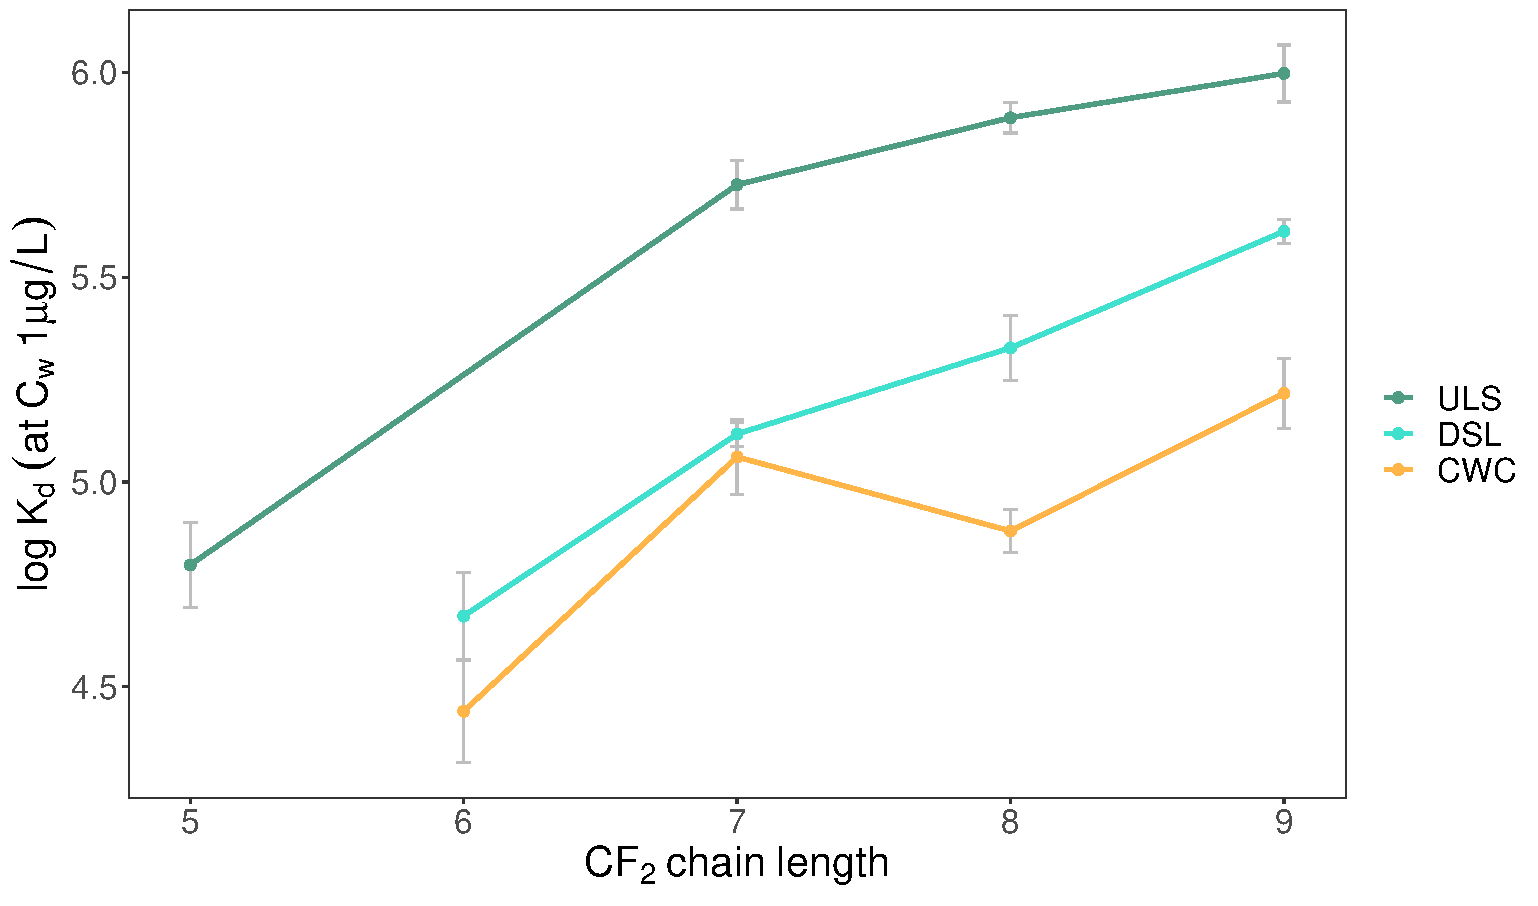
\includegraphics[width=0.7\textwidth]{R/figs/chain_length_Kd1ugL_plot.pdf}
    \caption{Relationship between $\log~K_F$ and chain length. Linear regression coefficients for ULS: $r^2$ = 0.92, $p$ = 0.04, DSL: $r^2$ = 0.98, $p$ = 0.01, CWC: $r^2$ = 0.68, $p$ = 0.17. Error bars are the propagated error of $\log~K_F$ and $n_F$.}
    \label{fig:chainlength}
\end{figure}

\subsubsection{PFAS functional groups} 
With the positive correlation between chain-length and PFCA sorption found in this study (\cref{fig:chainlength}), electrostatic interactions by the negatively charged carboxylate functional group seem to be of lesser importance. However, the effect of the charge-assisted polar head, especially for short-chain PFAS, cannot be disregarded. PFAS can engage simultaneously in hydrophobic interactions (perfluorinated chain) and in electrostatic interactions (attraction and repulsion), with both surface functional groups and dissolved ions (head) \citep{zhang2013sorption,sigmund2022sorption}. The different electrostatic interactions (cation bridging, biochar surface attraction and repulsion) are discussed more in depth in \cref{sec:inorganic}.

\cite{zhang2021sorption} found that sorption increased in the order PFBA $<$ PFBS $<$ PFOA $<$ PFOS for granular activated carbon and softwood-derived biochar. The difference between the PFSA and PFCA groups is that PFSAs have one more perfluorinated carbon than PFCAs, which have their terminal carbon bonded as a carboxylate (COO\textsuperscript{-}) instead of an additional $\mathrm{CF_2}$ moiety. If one compares PFHpS to PFOA, which both have the same number of $\mathrm{CF_2}$ moieties, perfluorinated sulfonic acid still sorbs better. Researchers attribute this to: 1) A difference in molecular size because the sulfonate moiety is slightly larger than the carboxylate moiety. This results in a greater cavity formation energy for PFSAs. Hence, in water saturated conditions, the functional group is pushed towards water extremities \citep{yin2022insights,sigmund2022sorption}. In batch shaking experiments, the water extremities would be the biochar surfaces or labware. 2) Sulfonic acid is a stronger acid than carboxylic acid. This results in a stronger ionic interaction to positive charges of mineral phases in biochar ash \citep{arvaniti2015review}. 

%%%%%%%%%%%%%%%%%%%%%%%%%%%%%%%%%%%%%%%%%%%%%%%%%%%%%%%%%%%%%%%%%%%%%%%%%%%%%%%%%%%%%%%%%%%%%%%%%%%%%%%%%%%%%%%%%%%%%%%%%%%%%%%%%%%%%%%%%%%%%%%%%%%%%%%%%%%%%%%%%%%%%%%%%%%%%%%%%%%%%%%%%%%%%%%%%%%%%%%%%%%%%%%%%%%%%%%%%%%%%%%%%%%%%%%%%%%%%%%%%%%%%%%%%%%%%%%%%%%%%%%%%%%%%%%%%%%%%%%%%%%%%%%%%%%%%%%%%%%%%%%%%%%%%%%%%%%%%%%%%%%%%%%%%%%%%%%%%%%%%%%%%%%%%%%%%%%%%%%%%%%%%%%%%%%%%%%%%%%%%%%%%%%%%%%%%%%%%%%%%%%%%%%%%%%%%%%%%%%%%%%%%%%%%%%%%%%%%%%%%%%%%%%%%%%%%%%%%%%%%%%%%%%%%%%%%%%%%%%%%%%%%%%%%%%%%%%%%%%%%%%%%%%%%%%%%%%%%%%%%%%%%%%%%%%%%%%%%%%%%%%%

\section{The effect of biochar properties on sorption}
In this section, the distribution coefficients derived for ULS, DSL and CWC biochars will be considered in relation to the following BC characteristics in an attempt to gain insight into possible sorption mechanisms: main elements (C, H, O, N), trace elements (Ca and Fe), surface area (\acrshort{SA}), and pore volume (\acrshort{PV}). In comparing sorbent properties and sorption coefficients for each biochar feedstock, PFOA, PFNA and PFDA have been used because they exhibited the best sorption isotherms. The Freundlich coefficients ($\log~K_F$) have been normalized to 1 $\mathrm{\mu g~L^{-1}}$ which is used as the distribution coefficient ($K_d$) in this discussion. Conducting multivariate analyses between biochar $K_d$ and the different supporting parameters for the biochar samples was desirable, but not statistically valid due to there being no degrees of freedom with only 3 samples. Therefore, the discussion on the effects of biochar properties on sorption will be limited to discerning trends with SA, PV, C, Ca and Fe. 

\subsection{Surface area and pore volume}\label{sec:SAPV}

\begin{table}
\centering
\caption{Surface area (SA), pore volume (PV), element content (C, O, H, N), and ratios for the biochars evaluated in the laboratory experiments.}
\adjustbox{max width=\textwidth}{
\label{tab:SAPV}
\begin{tabular}{lcccccccccccc}
\toprule
Biochar & \multicolumn{2}{l}{N\textsubscript{2} sorption} & \multicolumn{2}{l}{CO\textsubscript{2} sorption} & \multicolumn{4}{l}{Elemental content} & \multicolumn{3}{c}{Element ratio} \\
sorbent & \multicolumn{2}{l}{(pores \textgreater 1.5 nm)} & \multicolumn{2}{l}{(pores 0.4-1.5 nm)} & & & & & & \\ \cmidrule(l){2-3} \cmidrule(l){4-5} \cmidrule(l){6-9} \cmidrule(l){10-12} 
& BET SA  & BJH PV  & DFT SA & DFT PV & C & O & H & N & O/C & H/C & N/C \\
& ($\mathrm{m^2~g^{-1}}$) & (cm\textsuperscript{3} g\textsuperscript{-1}) & ($\mathrm{m^2~g^{-1}}$) & (cm\textsuperscript{3} g\textsuperscript{-1}) & (\%) & (\%) & (\%) & (\%) & & & \\ \midrule
CWC & 323 & 0.017 & 683 & 0.186 & 91.4 & 5.50 & 1.01 & 0.69 & 0.06 & 0.01 & 0.008 \\
ULS & 128 & 0.126 & 165 & 0.047 & 29.6 & 57.1 & 1.24 & 1.13 & 1.9  & 0.04 & 0.04 \\
DSL & 110 & 0.111 & 87  & 0.027 & 13.5 & 61.4 & 1.05 & 0.82 & 4.6  & 0.08 & 0.06 \\ \bottomrule
\end{tabular}}
\end{table}

\subsubsection{Pore size distribution between 0.4-1.5 nm}
\cref{tab:SAPV} shows the total surface area (SA, m\textsuperscript{2}/g) and pore volume (PV, cm\textsuperscript{3}/g) for the three biochars used in the sorption experiments in this study. SA of CWC biochar (683 m\textsuperscript{2} g\textsuperscript{-1}) was $\sim$six times higher than that of ULS and DSL biochars (165 and 87  m\textsuperscript{2} g\textsuperscript{-1}, respectively), and PV followed the same pattern. Previous research has postulated that large internal surface areas and pore volumes are desirable for strong sorption of organic contaminants because they increase the fraction of active sorption sites \citep{ahmed2020per,Hale2016}. The high SA and PV of CWC suggests that this biochar has the highest fraction of active sites compared to ULS and DSL biochars within the micropore range ($\le$ 2 nm). However, for SA and PV, the pore size distribution (PSD) of pores available for CO\textsubscript{2} adsorption (0.4-1.5 nm), shown in \cref{fig:PZD_small}, makes clear that nearly 80\% of the SA, and 60\% of the PV of CWC biochar, are located in pores smaller than 0.6 nm. These are referred to as ultra micropores \citep{bardestani2019experimental}. To find out whether PFCAs can be absorbed into these ultra micropores, \cref{tab:molecsize} lists effective cross-sectional diameter ($D_{eff}$) and maximum diameter ($D_{max}$) of each PFCA (the definitions of $D_{eff}$ and $D_{max}$ are illustrated in \cref{fig:molecularSize}). PFCAs C5-C10 range from 0.45-0.72 nm ($D_{eff}$) to 0.96-1.54 nm ($D_{max}$). Since the respective perfluorinated chains are too large and rigid to enter, most pores ($<$ 0.6 nm) turned out to be inaccessible to the PFCA molecules \citep{yu2009sorption}. In addition, pores that are too small make it difficult for the compounds to adjust their shape to the pore walls in order to be able to come close enough to sorb to the biochar surface. This is why they can get stuck in a cross-sectional position that blocks the pores for diffusion of new sorbates. 

Maximum sorption is achieved when the molecular dimensions of PFAS match the pore size and shape of the sorbent \citep{Hale2016}. Since the \acrshort{PSD} within the CO\textsubscript{2}-range is dominated by ultra micropores, sorption of PFPeA, PFHxA, and PFHpA is only possible if the congeners enter the pores at the exact right angle. PFOA, PFNA, and PFDA will experience size exclusion as their molecules are too large to sorb into the biochar pores in any direction (\cref{tab:molecsize}). This means that sorption of PFAS in the CO\textsubscript{2}-range is insignificant, and cannot explain the differences in the $\log~K_F$ obtained for the biochar feedstocks, especially since strongest sorption was measured for long-chain PFCAs.

\begin{figure}[htb]
    \centering
    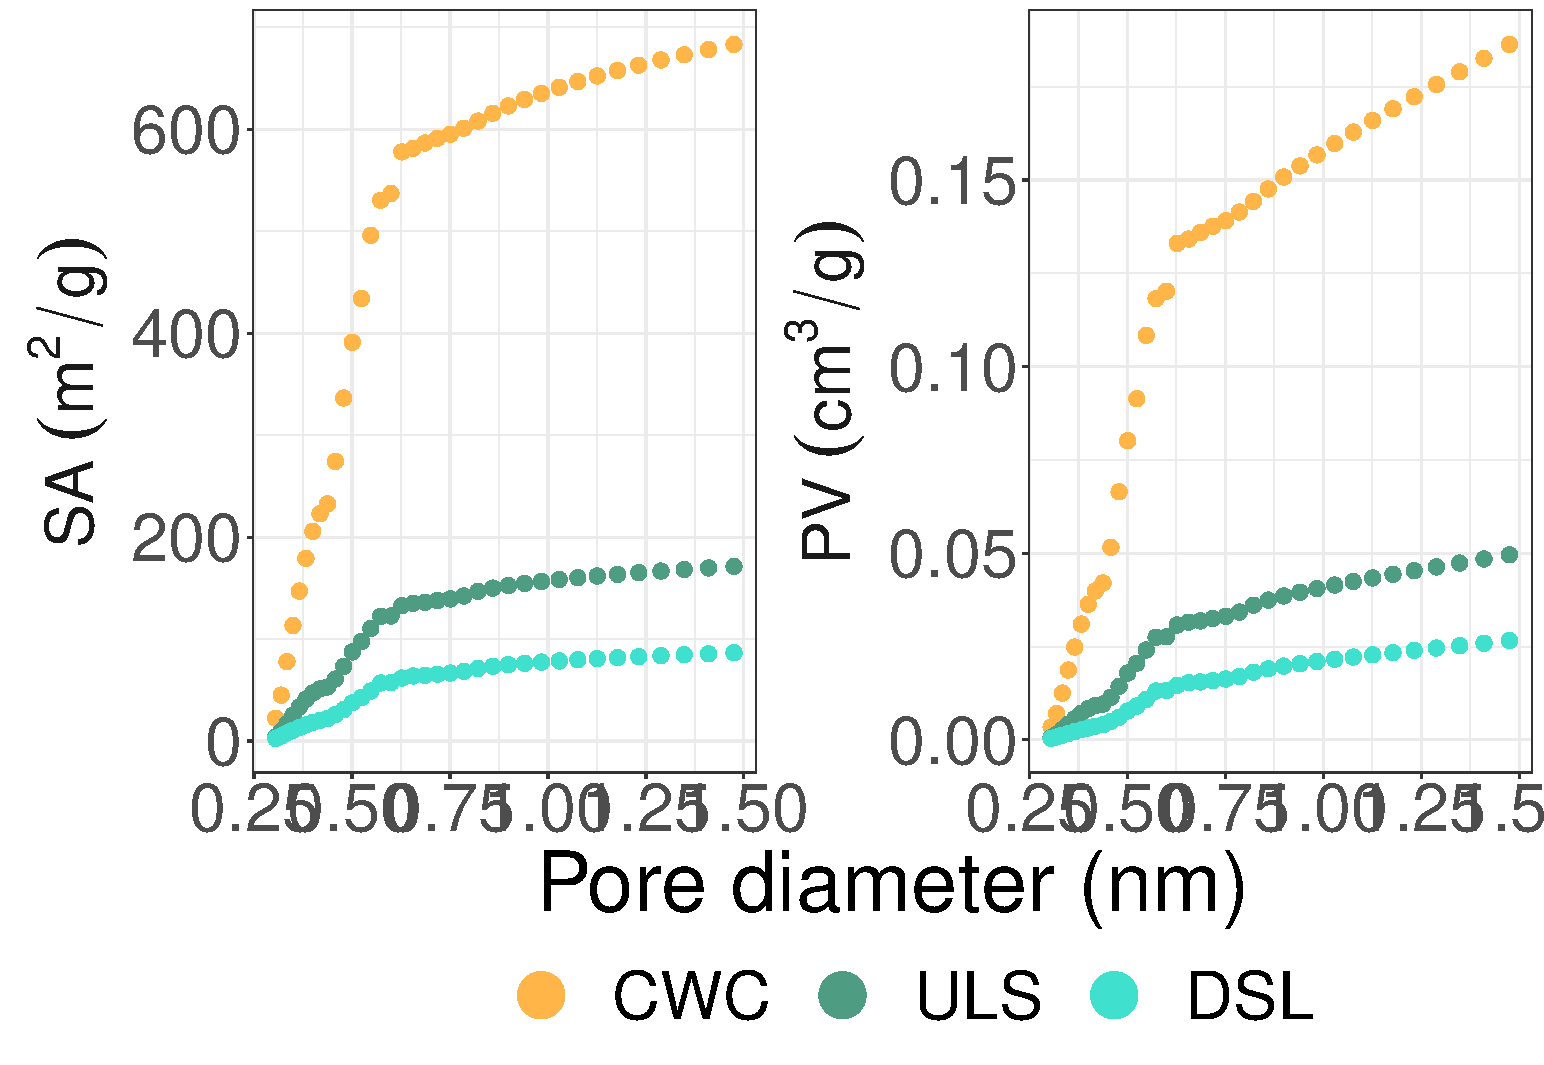
\includegraphics[width=\textwidth]{R/figs/PZD_SA_PV_small_plot.pdf}
    \caption{Cumulative pore size distribution for 0.4-1.5 nm-sized pores using DFT with (a) surface area (SA) and (b) pore volume (PV).}
    \label{fig:PZD_small}
\end{figure}

\begin{table}
\caption{Effective cross-sectional diameter ($D_{eff}$) and maximum diameter ($D_{max}$) of TCs interpolated and extrapolated by linear regression from calculations performed by \cite{inoue2012size} on PFOA and other PFCAs with chain lengths 11-18.}
\centering
\begin{threeparttable}
\label{tab:molecsize}
\begin{tabular}{lcrr}
\toprule
Compound & Chain & $D_{eff}$ & $D_{max}$ \\ 
& length & (nm) & (nm) \\ \midrule
PFPeA & 5  & 0.45  & 0.96  \\
PFHxA & 6  & 0.50  & 1.08  \\
PFHpA & 7  & 0.56  & 1.19  \\
PFOA\textsuperscript{*} & 8 & 0.61 & 1.36 \\
PFNA & 9 & 0.67 & 1.42  \\
PFDA & 10 & 0.72 & 1.54  \\ \bottomrule                                    
\end{tabular}
\begin{tablenotes}
\item \textsuperscript{*} Value from \cite{inoue2012size}
\end{tablenotes}
\end{threeparttable}
\end{table}

\begin{figure}
    \centering
    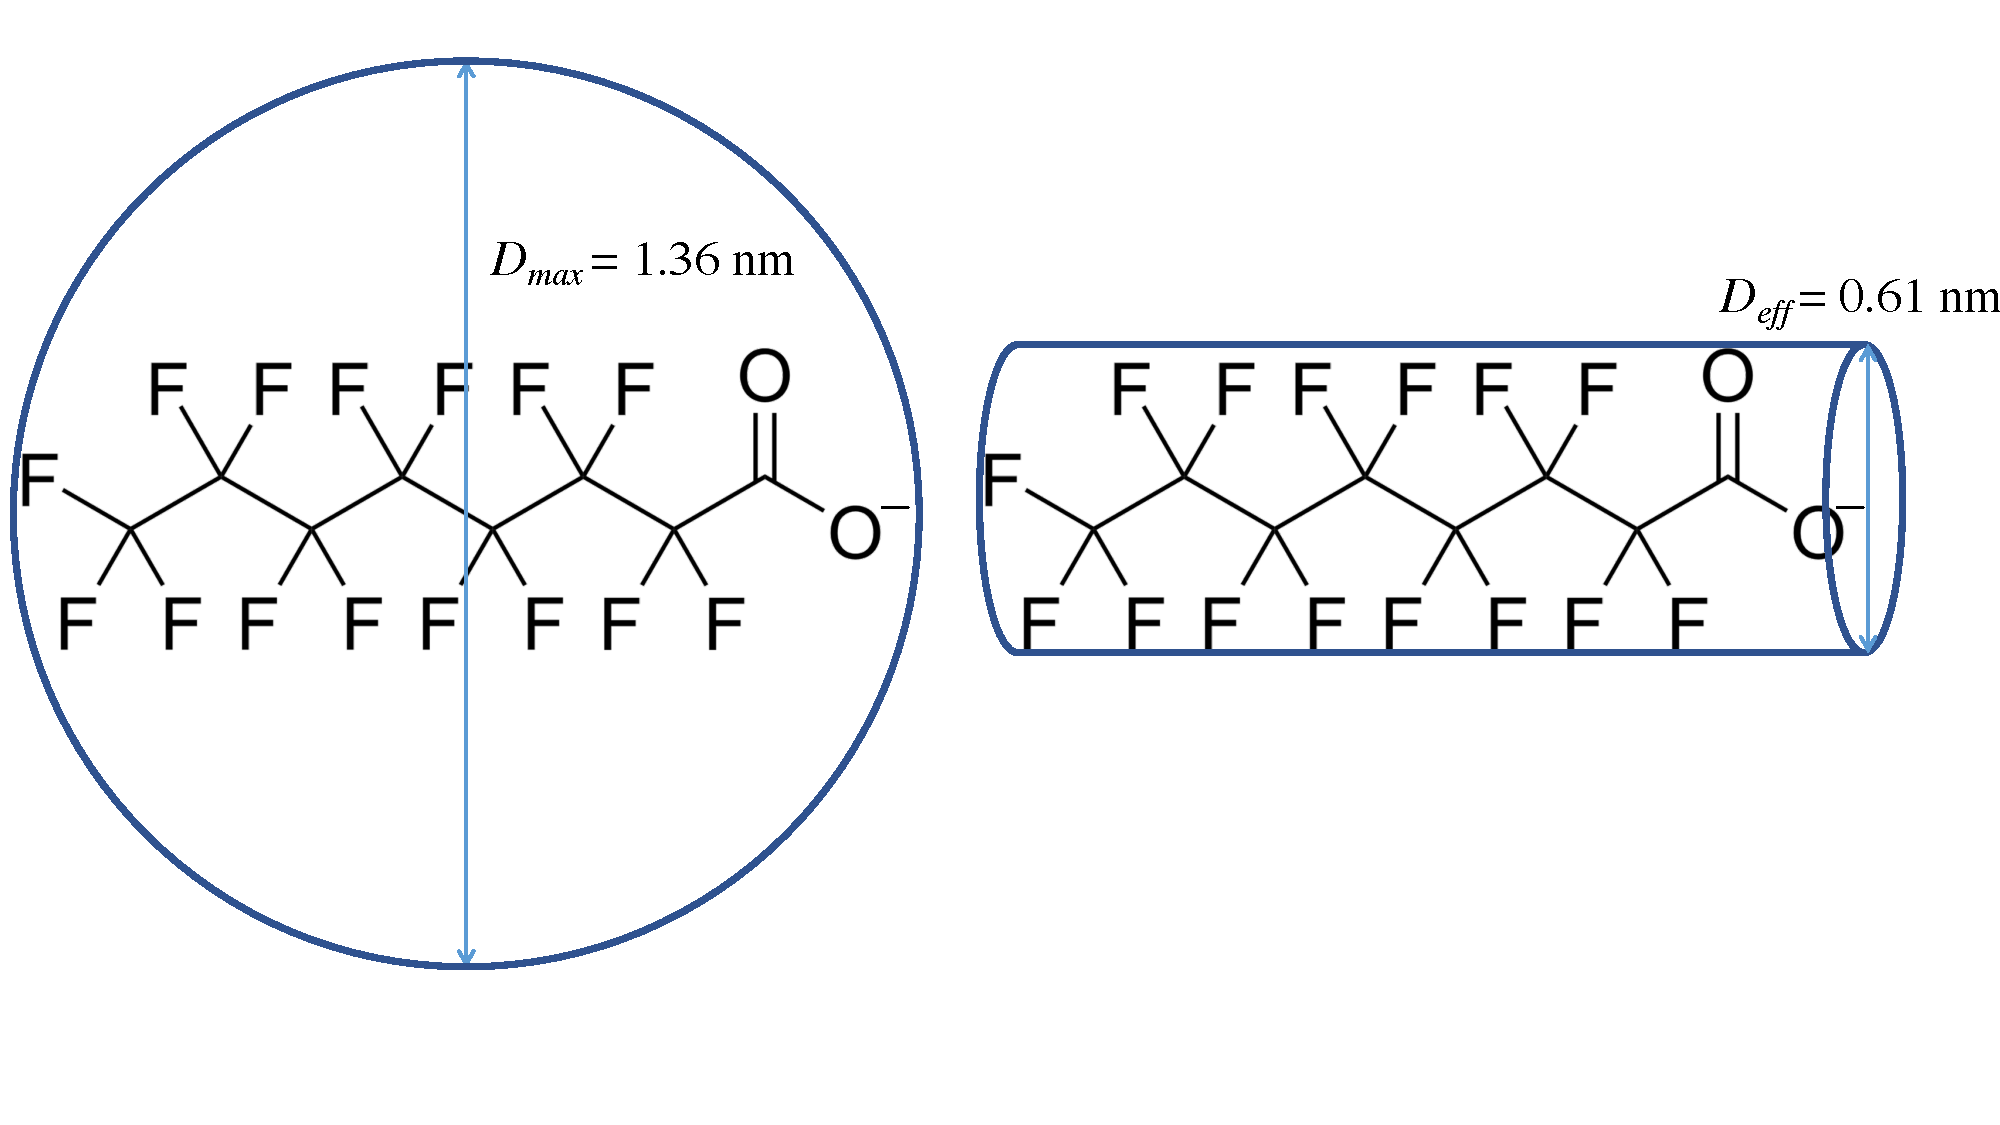
\includegraphics[width=0.8\textwidth, trim={0 2cm 0 0},clip]{Diagrams/Molecular_size.pdf}
    \caption{Effective cross-sectional diameter ($D_{eff}$) and maximum diameter ($D_{max}$) of PFOA.}
    \label{fig:molecularSize}
\end{figure}

\subsubsection{Pore size distribution for pores $>$1.5 nm}
CWC biochar had the largest cumulative SA (323 m\textsuperscript{2} g\textsuperscript{-1}), but the lowest PV (0.017 cm\textsuperscript{3} g\textsuperscript{-1}) for pores $>$1.5 nm. ULS biochar had slightly larger SA than DSL biochar (128 versus 110 m\textsuperscript{2} g\textsuperscript{-1}), as well as a slightly larger PV (0.126 versus 0.111 cm\textsuperscript{3} g\textsuperscript{-1}). In addition, the pore size distributions in \cref{fig:PZD_large} show remarkable differences in how SA and PV are distributed with increasing pore diameters between CWC biochar and the sludge biochars. For CWC biochar, SA and PV are almost exclusively allocated to pores between 1.5-3 nm. By contrast, SA and PV for the ULS and DSL biochars increase steadily up to a maximum pore size of 35 nm. Since ULS biochar has only slightly larger porosity compared to DSL biochar (\cref{fig:PZD_large}), the higher carbon content in ULS biochar (30 \% versus 14 \%) than DSL biochar indicates that more hydrophobic interactions are possible for ULS biochar. The difference in carbon content between ULS and DSL biochars is the most plausible explanation for why ULS biochar sorbs better than DSL biochar.. 

Apart from SA and PV, carbon content has, in previous literature, been a good predictor of sorption affinity to PFAS \citep{Hale2016, Cornelissen2005}. 

Three important conclusions can be drawn from this information: 1) CWC biochar has pores that are predominantly too small to accommodate PFCA, 2) CWC biochar has much lower PV for pores $>$1.5 nm, and this greatly restricts pore filling mechanisms, and 3) ULS biochar has a higher PV, SA and C-content than DSL biochar. This probably explains why ULS biochar is a better sorbent than DSL. In this study, the most plausible explanation for why CWC biochar is the weakest sorbent among the three biochars is that CWC biochar consists almost exclusively of micropores, whereas the ULS and DSL biochars have many more pores in the mesopore range (2-50 nm). This means that high porosity, and sufficiently large pores, are the two most important parameters that regulate high sorption capacity, and that a carbon-rich pore wall enhances sorption by increasing hydrophobic interactions. 

\begin{figure}[htb]
    \centering
    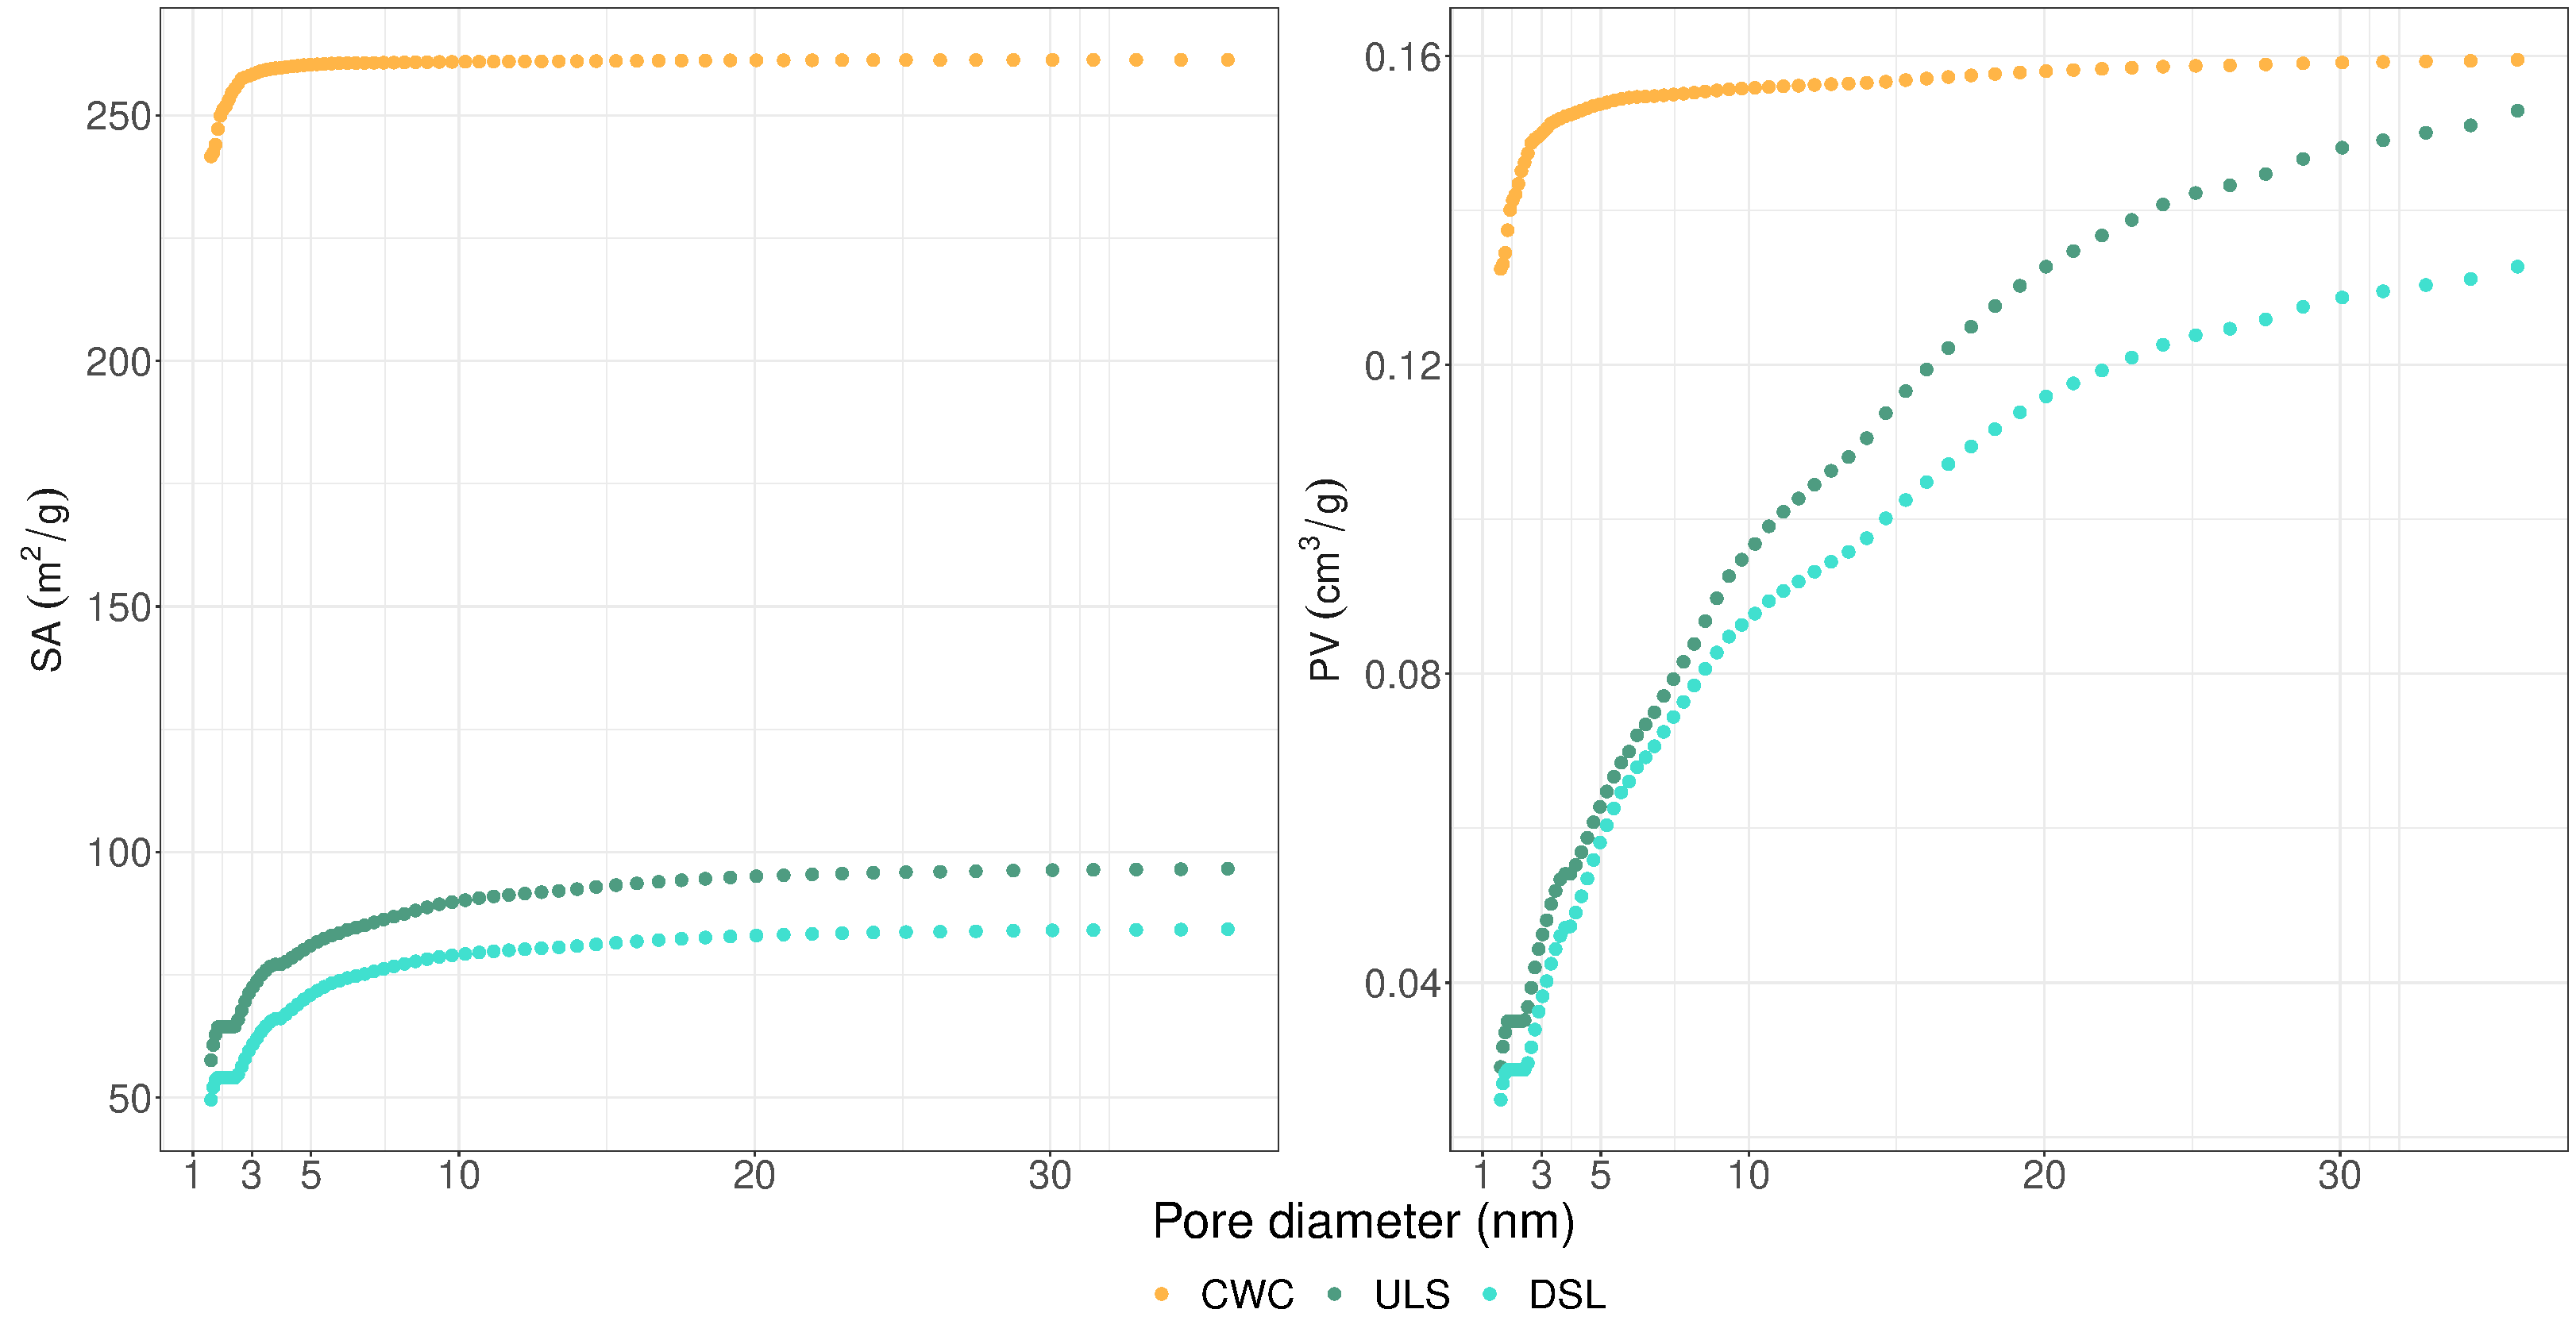
\includegraphics[width=\textwidth]{R/figs/PZD_SA_PV_plot_large.pdf}
    \caption{Cumulative pore size distribution for pores $>$ 1.5 nm using DFT theory with (a) surface area (SA) and (b) pore volume (PV).}
    \label{fig:PZD_large}
\end{figure}

\subsection{Biochar surface chemistry}
A higher carbon fraction is commonly used as an indicator of biochar aromaticity and, thereby, gives biochar a higher possibility for hydrophobic interactions \citep{Cornelissen2005}. The higher sorption of PFCAs to the ULS and DSL biochars stand in contrast to findings in previous literature that consistently report that higher C-content is a good predictor for increased sorption \citep{fabregat2022examining}. However, previous PFAS sorption studies have been conducted on activated biochar and charcoal, more carbon-rich and porous feedstocks than biochar from sewage sludge \citep{Sormo2021, zhang2021sorption}. Despite lower carbon contents in the ULS and DSL biochars, this study supports previous literature that concluded that the importance of electrostatic interaction to sorption is secondary to the hydrophobic effect. 

Surface hydrophobicity and degree of carbonization can be described by O/C, H/C, and N/C ratios \citep{chun2004compositions}. As reported previously, the O/C ratio of CWC (0.06) is within the same range as non-activated biochars pyrolyzed at 700\textdegree C \citep{LehmannAndJoseph2015, chun2004compositions,kupryianchyk2016biochar}. By contrast, the high oxygen content of DSL and ULS (61.4 and 57.1 \% respectively) results in increased O/C ratios of 4.6 and 1.9 respectively (\cref{tab:SAPV}). The difference between the O/C ratio \textless 1 for CWC compared to ratios \textgreater 1 for ULS and DSL indicate a significantly different degree of carbonization between the two feedstock types. At the same time, H/C ratios for all three biochar feedstocks are similar, and are within the same range reported in previous literature \citep{chun2004compositions,kupryianchyk2016biochar}. 

A higher O/C and N/C ratio---indicative of more polar functional groups (hydroxyl, carbonyl, metal-containing groups, amines and amides)---has proven to be beneficial for PFAS sorption \citep{du2014adsorption,fabregat2022examining}. Researchers suggest several mechanisms related to surface polar groups that may contribute to enhanced sorption. First, basic functional groups such as amines have high $pK_a$s and are protonated at environmentally relevant pH levels, providing anion exchange capacity and electrostatic attraction to the carboxylic acid heads \citep{deng2010removal}. Basic sites in \textpi-electron-rich, carbon-rich materials are important for PFAS sorption \citep{saeidi2020understanding}. N/C ratios for ULS and DSL are one order of magnitude higher than CWC. A high nitrogen/carbon (N/C) ratio can be indicative of more amine groups in the periphery of the condensed carbon structure. The positive charge on the nitrogen-containing functional groups can interact electrostatically with the PFCA carboxylate group. In addition, it is possible that they also engage in weak non-specific electrostatic interactions with the negative dipole of the CF-chain \citep{xiao2011effects}. The latter mechanism could explain the positive chain-length dependency on sorption seen for the sewage sludge biochars (\cref{fig:chainlength}), in addition to the low SA/PV/C ratio discussed in the previous section. Sewage sludge contains a homogeneous mixture of proteins and inorganic nutrients that will denaturate in some form during thermal treatment. To the author's knowledge, no data exists on how speciation of nitrogen changes during pyrolysis. Even though a higher N/C ratio is only an indication for nitrogen functional groups, the presence of amines is likely.

\begin{table}
\centering
\caption{Mean pH ($\pm$ standard error) measurements for the different batch test slurries (n=3) where S is soil and BC/S/L is the biochar:soil:liquid ratio.}
\label{tab:pHcond}
\begin{tabular}{lcc}
\toprule
Biochar & \multicolumn{1}{c}{pH} & BC/S/L\\ \midrule
ULS   & 7.10 ± 0.03 & 1/0/500\\
DSL   & 7.31 ± 0.01 & 1/0/500\\
CWC   & 7.36 ± 0.04 & 1/0/500\\
ULS+S & 7.18 ± 0.01 & 1/50/500\\
DSL+S & 7.14 ± 0.00 & 1/50/500\\
CWC+S & 7.09 ± 0.03 & 1/50/500\\
S     & 7.08 ± 0.03 & 0/1/10\\
\bottomrule
\end{tabular}
\end{table}


\subsubsection{Solution and biochar surface chemistry \label{sec:inorganic}} 
Solution chemistry, pH, and the composition of elements other than C, O, H and N, may provide further insight into how the pore walls of CWC, ULS and DSL differ from one another, as well as how these elements can influence sorption. pH varied little across sample types with an average pH of 7.18 $\pm$ 0.02 (\cref{tab:pHcond}). Therefore, pH levels for the biochar-water batch tests slurries have only been used to discuss expected surface charges. In the environment, the carboxylic functional group of PFCAs is negatively charged due to the strong electron-withdrawing fluorine atoms \citep{goss2008pKa}. Surface charges for biochar are pH-dependent, and are usually negatively charged at a neutral pH \citep{zhang2013sorption}. This was the case for the batch tests in the present study. However, point-of-zero charge measurements for the biochars did not become available in time for incorporation in this discussion. Therefore, a net negative biochar surface is assumed, but not confirmed \citep{saeidi2020understanding}.

In this study, highest sorption was seen for the biochars that had the highest composition of elements other than C, O, H, and N. CWC biochar contained only 1.4\% of other elements, whereas the sludge biochars, ULS and DSL, contained substantially more (10.9\% and 23.2\% respectively). A table with the total biochar elemental composition is given in \cref{appSec:elements}. Some of these elements are commonly found as freely dissolved ions. Since dissolved ions were not analyzed, we can only assume that, by and large, the alkalis (K and Na), and earth alkalis (Mg and Ca), are present as dissolved cations that originate from the biochar ashes. It is likely that Fe is predominantly incorporated in the biochar matrix. Iron speciation will be further discussed in \cref{sec:Fe}. The higher content of other elements than C, H, O, and N in ULS and DSL biochars suggests that sorption of PFCAs onto the sludge chars were likely influenced by the presence of charged species, both in the solution, as well as on the biochar surface. Coexisting inorganic ions complicate the sorption behavior of PFCAs because sorption can both be suppressed and enhanced by different electrostatic mechanisms \citep{du2014adsorption}. This will be discussed below. 

Sorption can be suppressed by electrostatic repulsion of the carboxylate group on PFCA by the negatively charged biochar surface, or by competitive sorption of anions to positive BC sites \citep{sigmund2022sorption}. Electrostatic repulsion explains why $K_F$-values were lowest for the shorter-chain PFCAs (\cref{tab:summary_stats_single}). The repulsion effect becomes weaker for the longer-chain PFCAs where the hydrophobic effect become more dominant. Electrostatic repulsion is reduced at lower pH because more negative BC sites are protonated, a process called surface-charge neutralization \citep{zhang2013sorption}. This allows for PFCA anion- \textpi-bond interaction with biochar \citep{sigmund2022sorption}. Sorption can be enhanced through electrostatic attraction to positively charged BC functional groups, and by divalent cation bridging \citep{du2014adsorption}. Cation bridging is the electrostatic linking of negatively charged PFCAs to negatively charged biochar surfaces by means of a divalent ion that acts as a "bridge" between them \citep{sigmund2022sorption}. Ca\textsuperscript{2+} and Mg\textsuperscript{2+} are common divalent ions present in biochar ash that contribute to bridging. The composition of Ca\textsuperscript{2+} and Mg\textsuperscript{2+} was three to six times higher in the sludge biochars when compared to CWC biochar (\cref{tab:BC_mainElements}. 

Bridging has been shown to be an important sorption mechanism in, for example, sediments, mineral materials, and black carbon \citep{higgins2006sorption}. Apart from bridging between the BC surface and PFAS functional groups, divalent ions can chain individual PFAS molecules together \citep{wang2011}. This creates an even more hydrophobic complex that can sorb more strongly to biochar. For this reason, more frequent formation of divalent cation bridges for the ULS and DSL biochars is expected. Although sorption \textit{capacity} has not been measured directly, the above mechanisms for PFAS interaction with charged and polar functional groups may be contributors to the higher sorption found for the more heterogeneous, mineral-rich matrices of sewage sludge biochars.

In this study, the positive correlation between $\log~K_F$ and chain length for all three biochars (\cref{fig:chainlength}) indicates that electrostatic interactions play a minor role for sorption to these biochars. If electrostatic interactions played an equally important role as hydrophobic interactions, sorption across differing PFCA chain lengths would be more similar. 

\begin{table}
\centering
\caption{Composition of a selection of elements in the biochar samples in g/kg.}
\label{tab:BC_mainElements}
\begin{tabular}{lrrrrrrrr} \toprule
 & Ca & Fe & K & Mg & Na & P & S & Si \\ \midrule
CWC & 8 & 0.1 & 4.0 & 0.9 & 0.05 & 0.4 & 0.09 & 0.2 \\
DSL & 26 & 180 & 3.7 & 4.7 & 1.8 & 8.0 & 7.2 & 0.6 \\
ULS & 21 & 23 & 6.8 & 5.3 & 2.4 & 45 & 2.9 & 1.7 \\ \bottomrule
\end{tabular}
\end{table}

\subsubsection{Iron speciation\label{sec:Fe}}
Due to a lack of corresponding reference compounds for some of the EXAFS signals, no satisfying fit was obtained for the iron species present in sewage sludge biochar samples. This suggests that iron is not only present as iron oxides. The Fe K-edge XANES spectra (\cref{appFig:valence}) and EXAFS spectra (\cref{appFig:Fe_species}) show that DSL and ULS are similar in valence and speciation. They consist mainly of reduced forms of Fe (Fe(II)), and DLS is slightly more reduced than ULS. Total Fe concentration is especially high for DSL (180 mg/kg, \cref{tab:BC_mainElements}), making up as much as 18\% of its matrix (3.3\% and 0.01\% for ULS and CWC respectively). The Fe concentration will therefore significantly affect the surface morphology of DSL. PFAS has been shown to form inner-sphere complexes via covalent metal-ligand bonds (Fe-carboxylate) by means of the following reaction \citep{du2014adsorption}:

\begin{equation}
    \mathrm{\equiv Fe-OH_2^+ ~ + ~ CF_3(CF_2)_nCOO^- \rightarrow ~ \equiv Fe-OOC(CF_2)_nCF_3 ~+~ H_2O}
\end{equation}

The triple bond represents chelation of Fe to the biochar matrix. Point of zero charge (PZC) for Fe(oxyhydr)oxides, such as ferrihydrite and goethite, are around 7, similar to the solution pH measured for the water-biochar systems (see \cref{sec:inorganic}). The iron species are expected to be neutral for the systems analyzed, and will likely not be one of the dominating sorption mechanisms for PFCA. 

%%%%%%%%%%%%%%%%%%%%%%%%%%%%%%%%%%%%%%%%%%%%%%%%%%%%%%%%%%%%%%%%%%%%%%%%%%%%%%%%%%%%%%%%%%%%%%%%%%%%%%%%%%%%%%%%%%%%%
%%%%%%%%%%%%%%%%%%%%%%%%%%%%%%%%%%%%%%%%%%%%%%%%%%%%%%%%%%%%%%%%%%%%%%%%%%%%%%%%%%%%%%%%%%%%%%%%%%%%%%%%%%%%%%%%%%%%%
%%%%%%%%%%%%%%%%%%%%%%%%%%%%%%%%%%%%%%%%%%%%%%%%%%%%%%%%%%%%%%%%%%%%%%%%%%%%%%%%%%%%%%%%%%%%%%%%%%%%%%%%%%%%%%%%%%%%%

\section{Sorption attenuation by soil and PFCA cocktail}
This section discusses sorption attenuation for the different batch test categories that were prepared (\cref{sec:batch}). In this study, the same equilibrium concentrations were not achieved across all samples. Therefore, $K_d$-values with the same \textit{total} concentrations were compared. \cref{subfig:C10} shows how much $K_d$ is suppressed by the presence of soil and/or a mixture of PFCAs at the highest spike point, SC10. A description of considerations that were taken for the determination of $K_d$ values in soil is in \cref{appSec:Sorption}, \cref{appsec:attenuation}. The difference in $\log~K_d$ between BC single and the other sample types is directly related to how much sorption was attenuated by the presence of soil and/or other PFCAs. As visualized by the order of the colored points, attenuation increased in the following order: BC-single (reference) $>$ BC-soil-single $>$ BC-mixed $\sim$ BC-soil-mixed $>$ soil-single and soil-mixed. Attenuation factors ($AF$) were calculated for each category:

\begin{equation} \label{eq:$AF$}
    AF = \frac{K_{BC-single}}{K_{BC-x}}
\end{equation}

where $K_{BC-single}$ is the expected sorption, and $K_{BC-x}$ is the measured partition coefficient for the mixed, soil-mixed, or soil-single batch tests. In \cref{subfig:$AF$}, the $AFs$ for PFOA, PFNA, and PFDA have been plotted for each biochar. $AFs$ ranged from 3-10 for BC-S-PFOA, 6-140 for BC-mix, and 8-138 for BC-S-mix (\cref{tab:attenuation}). The cocktail consisted of 18\% PFOA, 21\% PFNA, and 49\% PFDA (\cref{tab:spikeConcentrations}). Since the concentrations for each compound was different, and nearly 50\% of the cocktail was PFDA, PFNA and PFOA, likely were overwhelmed, showing that PFDA  a trend for attenuation with chain length cannot be derived. These factors are very high due to five other compounds added at similar concentrations with a total concentration of 10 mg/L. It was difficult to evaluate any trends in $AF$s between biochar samples or PFCA chain lengths, but PFDA does not seem to be overwhelmed... 

Since the $AFs$ varied widely within each category, mean and median values for each category were calculated to evaluate trends. BC-S-PFOA: mean = 6, median = 4, BC-mix: mean = 43, median = 29, and BC-S-mix: mean = 59, median = 49. Thus, attenuation for the cocktail samples was one to two orders of magnitude higher than attenuation by soil alone. The presence of soil with a cocktail caused additional attenuation of 27\% ($\mathrm{AF_{soil} = 59-43 = 16}$. These $AFs$ are in the same range as in previous literature where it was established that sorption was attenuated by a factor of 10 for phenanthrene by means of adding other PAHs \citep{Cornelissen2006}, 32 for a mixture of DDT \citep{hale2009sorption}, and 100-500 for sulfamethazine (SMT) in soil after \cite{Teixido2013}. The high attenuation for sulfamethazine seen by \cite{Teixido2013} is in the same order as the $AFs$ found in the present study. Sorption of both SMT (a structure  that consists of a sulfonamide functional group that links two aromatic rings with nitrogen-substitutions, methyls and an amine), and PFAS to biochar seems to be more affected by the presence of soil than does sorption of the hydrophobic organic contaminants (HOCs), phenanthrene and DDT. Though speculative, and taking into account that sorbents and conditions vary, this could indicate that HOCs can more easily penetrate the humic acid pore blockages than can PFAS and SMT. A hypothesis that could explain this is that SMT and PFAS are more similar in hydrophobicity as humic acids. This means that they share a level playing field in the competition for sorption sites. However, since humus is larger than PFAS, pores remain non-penetrable. A more extensive determination of structure-property relationships and attenuation would be needed to confirm this hypothesis. 

As a final note, one cannot know if the $AFs$ derived after 14 days in the present study would be reduced given increased soil-BC-mix and BC-water-mix contact times such as were seen by \cite{hale2009sorption} who found that attenuation of DDT disappeared ($AF$ = 1) after 26 months. A sorption capacity test would have to be conducted to determine if sorption sites for CWC, ULS, and DSL biochars truly were saturated and at equilibrium after 14 days for BC-mix without soil. Or whether diffusion and occupation of all sorption sites would increase with increased contact time. 

To the best of the author's knowledge, there are no existing attenuation factors for sewage sludge biochar to PFAS. Attenuation depends mainly on two factors: 1) sediment-BC contact time, and 2) concentration of cocktail. Since it was shown that soil did not contribute to further suppressed sorption, sorbents can, without difficulty, be amended to soil with low \acrshort{TOC} (1.3\%), such as the present one \citep{Sormo2021}.


\begin{table}
\centering
\caption{Attenuation factors ($AF$) calculated as $K_{BC_single}/K_{BC_x}$ and respective $\log~K_d$-values at SC10.}
\label{tab:attenuation}
\begin{tabular}{llrrrrrr} \toprule
Compound & type & \multicolumn{2}{c}{CWC} & \multicolumn{2}{c}{DSL} & \multicolumn{2}{c}{ULS} \\ \cmidrule(l){3-4} \cmidrule(l){5-6} \cmidrule(l){7-8}
 &  & $\log~K_d$ & $AF$ & $\log~K_d$ & $AF$ & $\log~K_d$ & $AF$ \\ \midrule
PFOA & BC-mix & 2.84 & 6 & 3.17 & 23 & 4.13 & 29 \\
PFNA & BC-mix & 2.33 & 109 & 3.03 & 140 & 4.40 & 29 \\
PFDA & BC-mix & 2.95 & 9 & 3.60 & 32 & 5.09 & 9 \\ \addlinespace \hline \addlinespace
PFOA & BC-S-mix & 2.73 & 8 & 3.24 & 19 & 3.47 & 134 \\
PFNA & BC-S-mix & 2.68 & 48 & 3.33 & 71 & 3.73 & 138 \\
PFDA & BC-S-mix & 2.91 & 10 & 3.67 & 27 & 4.16 & 78 \\ \addlinespace \hline \addlinespace
PFOA & BC-S-PFOA & 3.19 & 3 & 3.98 & 4 & 4.61 & 10 \\ \bottomrule
\end{tabular}
\end{table}


\begin{figure}
    \centering
        \begin{subfigure}[]{\linewidth}
            \centering
            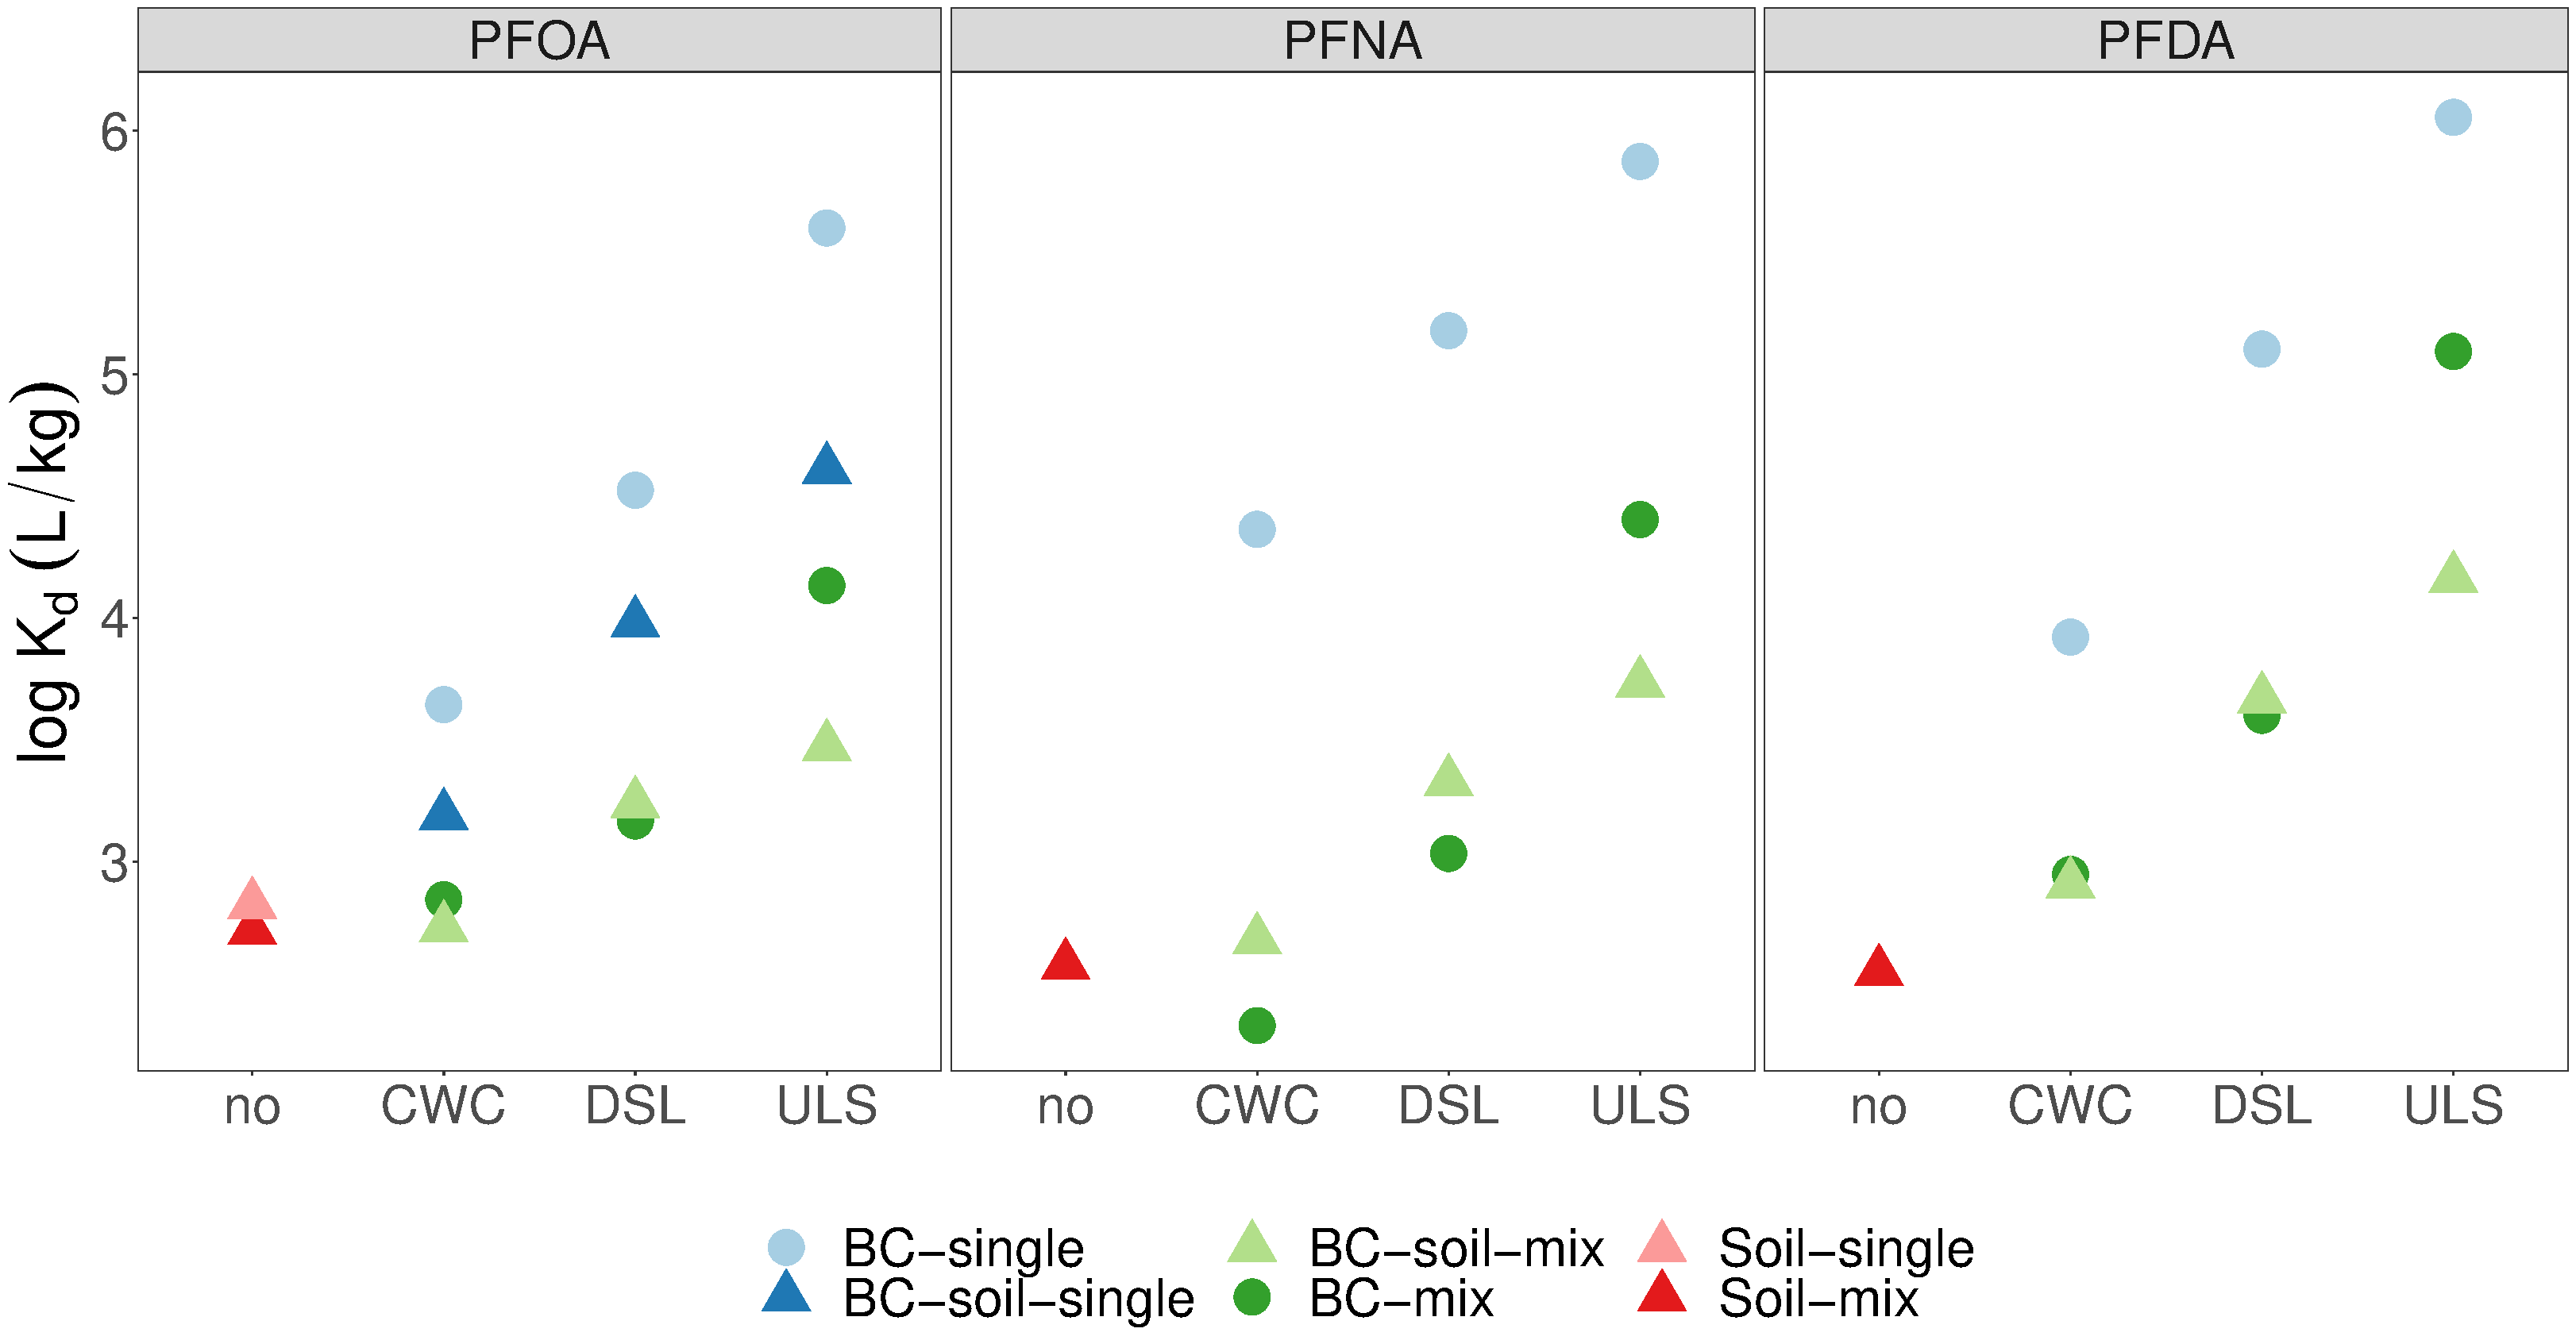
\includegraphics[width=0.9\textwidth]{R/figs/C10.pdf}
            \subcaption{$\log~K_d$ for PFOA, PFNA, and PFDA spiked at SC10 (1 953, 1 409, and 3 830 \textmu g L\textsuperscript{-1} respectively) for the different biochar feedstocks (CWC, DSL, ULS) and soil-only (no biochar). $\log~K_d$ for BC single (light blue circles) are the predicted sorption by biochar.\\}
            \label{subfig:C10}
        \end{subfigure}
        \begin{subfigure}[]{\linewidth}
            \centering
            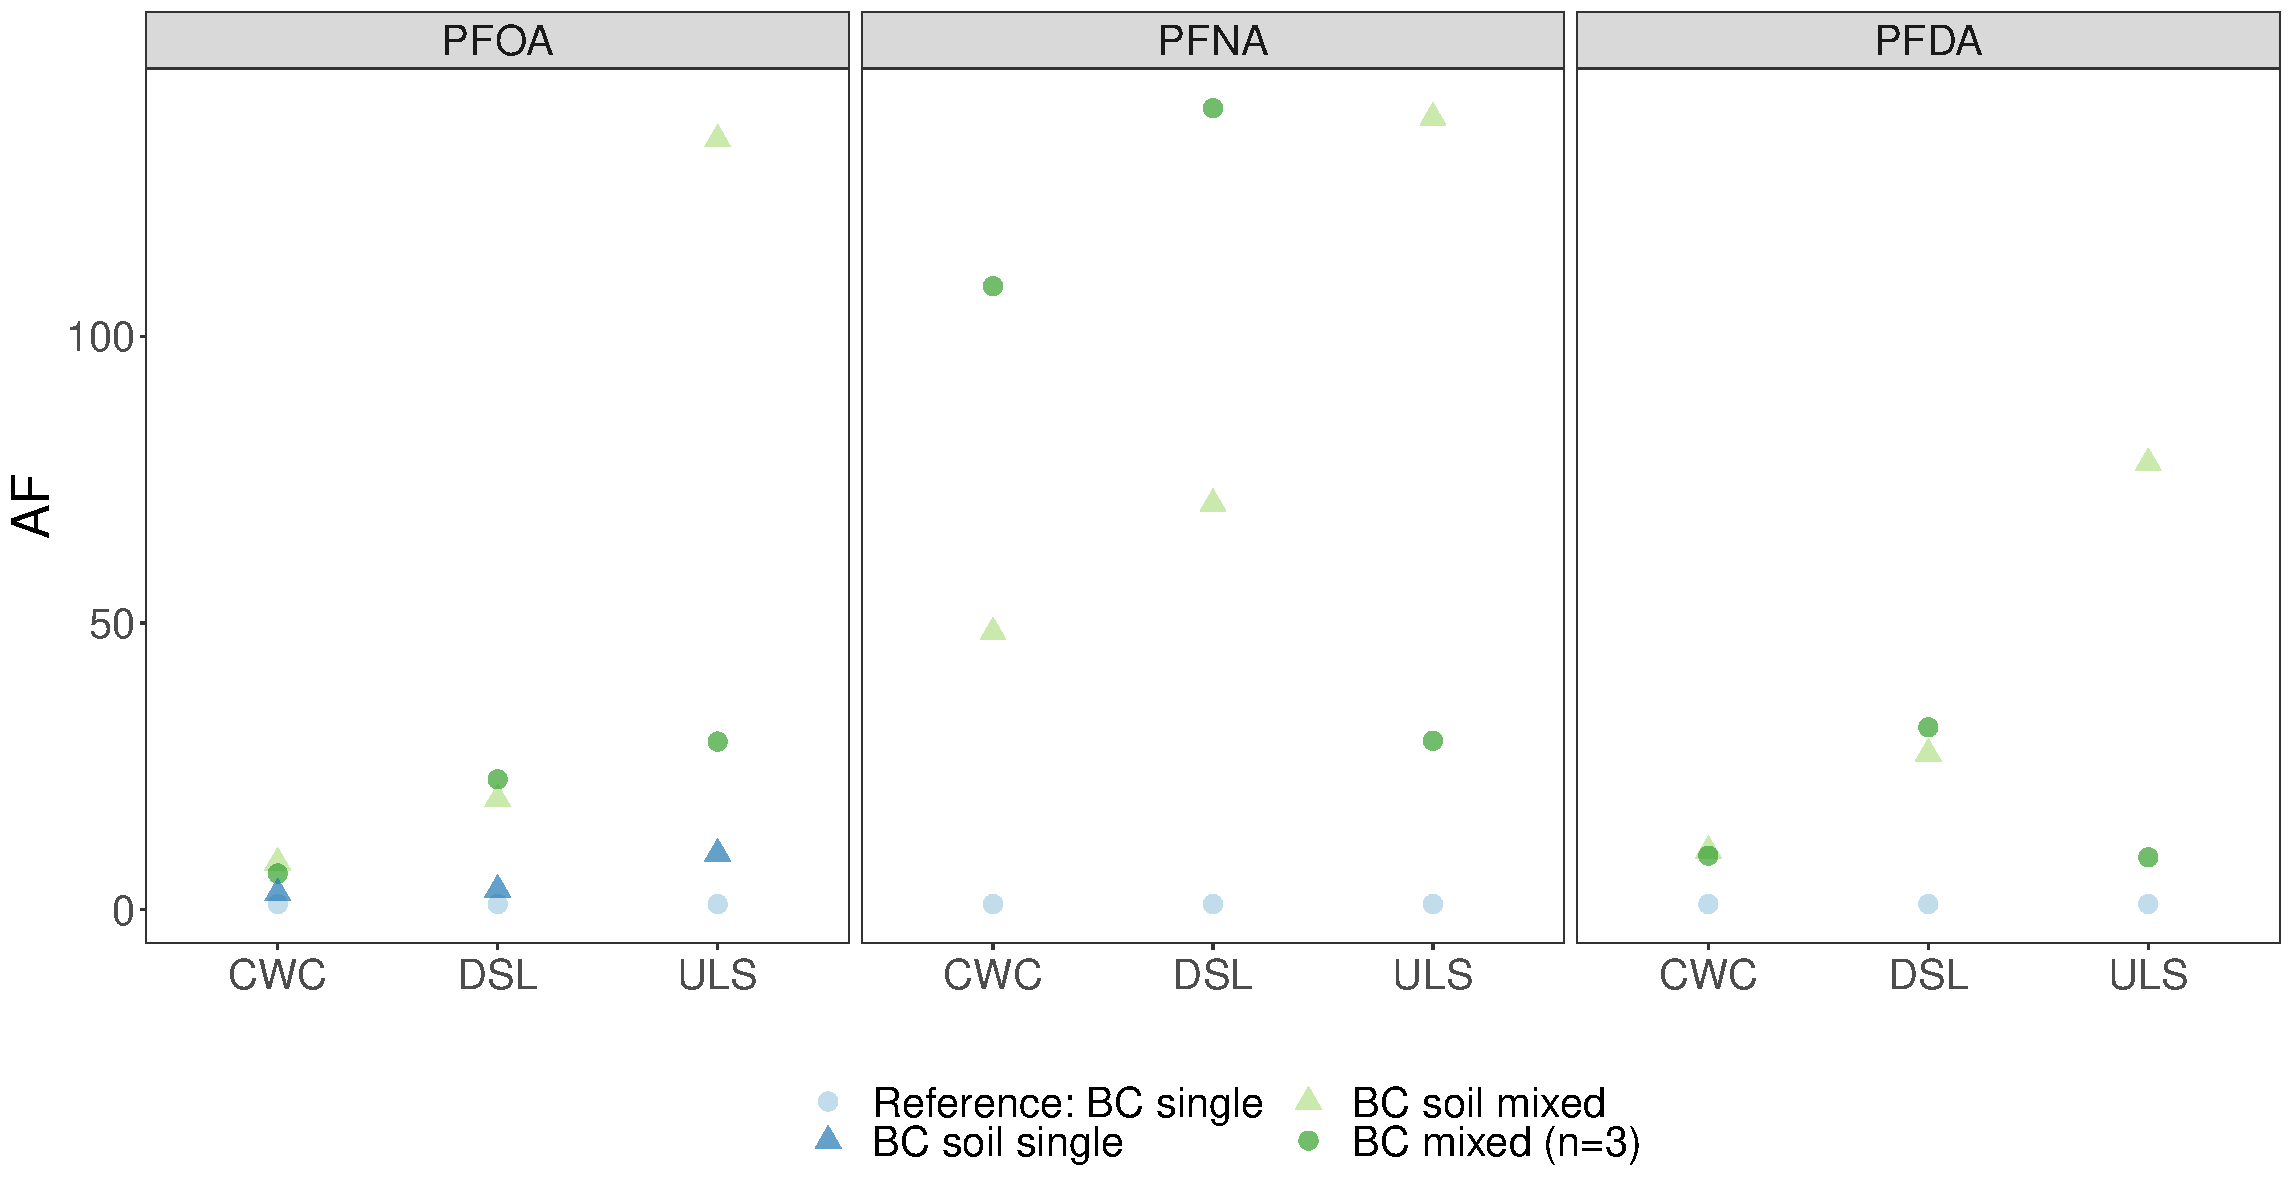
\includegraphics[width=0.9\textwidth]{R/figs/Attenuation_factors_C10_OND.pdf}
            \subcaption{Attenuation factors ($AF$) at SC10 for PFOA, PFNA, and PFDA calculated as $K_{d,BC single}/K_{d,x}$ where $K_{d,x}$ are batch test categories. See \cref{tab:spikeConcentrations} for spike concentrations used for each PFCA in the single-spike and cocktail-spike batch tests.}
            \label{subfig:$AF$}
        \end{subfigure}  
    \caption{Reduction in \textbf{(a)} $\log~K_d$ at SC10 and \textbf{(b)} attenuation factors at SC10.}
    \label{fig:C10_AF}
\end{figure}

\subsection{Sorption attenuation of PFOA isotherms}
\cref{fig:PFOA_attenuation} shows the effect of attenuation on the PFOA isotherms for BC soil single, and BC soil mixed. The isotherms were spiked with the same $C_i$ as BC single. But only six of the ten points were selected for the attenuation isotherms (\cref{sec:batch}. For all biochars, BC single has the highest sorption, followed by BC soil single, and BC soil mixed. This trend gives a good indication of the order of factors that influence attenuation, and is consistent with the results discussed in the previous section. The isotherms have similar $C_s$ concentrations, but varying $C_w$, depending on sample type. Due to pore blocking and competitive sorption by natural organic matter and natural compounds, more sorbate in solution is needed to push the same number of molecules onto the solid phase in the presence of soil, an effect that can be further enhanced by the presence of both soil and a cocktail since this isotherm has the highest $C_w$ and lowest $C_s$. This particular quality is due to the fact that PFCAs with longer chain lengths (PFNA and PFDA) have an advantage over PFOA when competing for sorption sites \citep{Sormo2021}. Supported by the trends in \cref{fig:C10_AF}, the cocktail attenuation effect is more significant than attenuation by soil. Parallel isotherms mean that attenuation is the same across the whole concentration range, as, for instance, between BC-single and BC-soil-single for ULS. For some isotherms, attenuation is minimal at low concentrations and increases with increasing spike concentration. This is the case for the DSL isotherms, and can be explained by the non-linear sorption at higher concentrations. So, when spike concentration increases, sorption attenuation also increases. 

\cite{siriwardena2019influence} measured attenuation factors for PFOA to two granulated activated carbons (GAC), one coal-based and one coconut-based. GAC is an adsorption media with extremely high internal surface area. It is produced from organic material such as coconut shells, coal, peat, or wood. The coal-based carbon had an $AF$ of 3.3 and the coconut-based carbon had an $AF$ of 1.7 in the presence of the co-contaminants, kerosene, ethanol, and trichloroethylene. The cumulative initial concentration used was 4.1 mg/L, half the total concentration spiked in the present study. $AFs$ of 23 and 29 for PFOA, in BC-mix for DSL and ULS respectively, (\cref{tab:attenuation}) are slightly higher than those found by \cite{siriwardena2019influence}. 

\begin{figure}[htb]
    \centering
    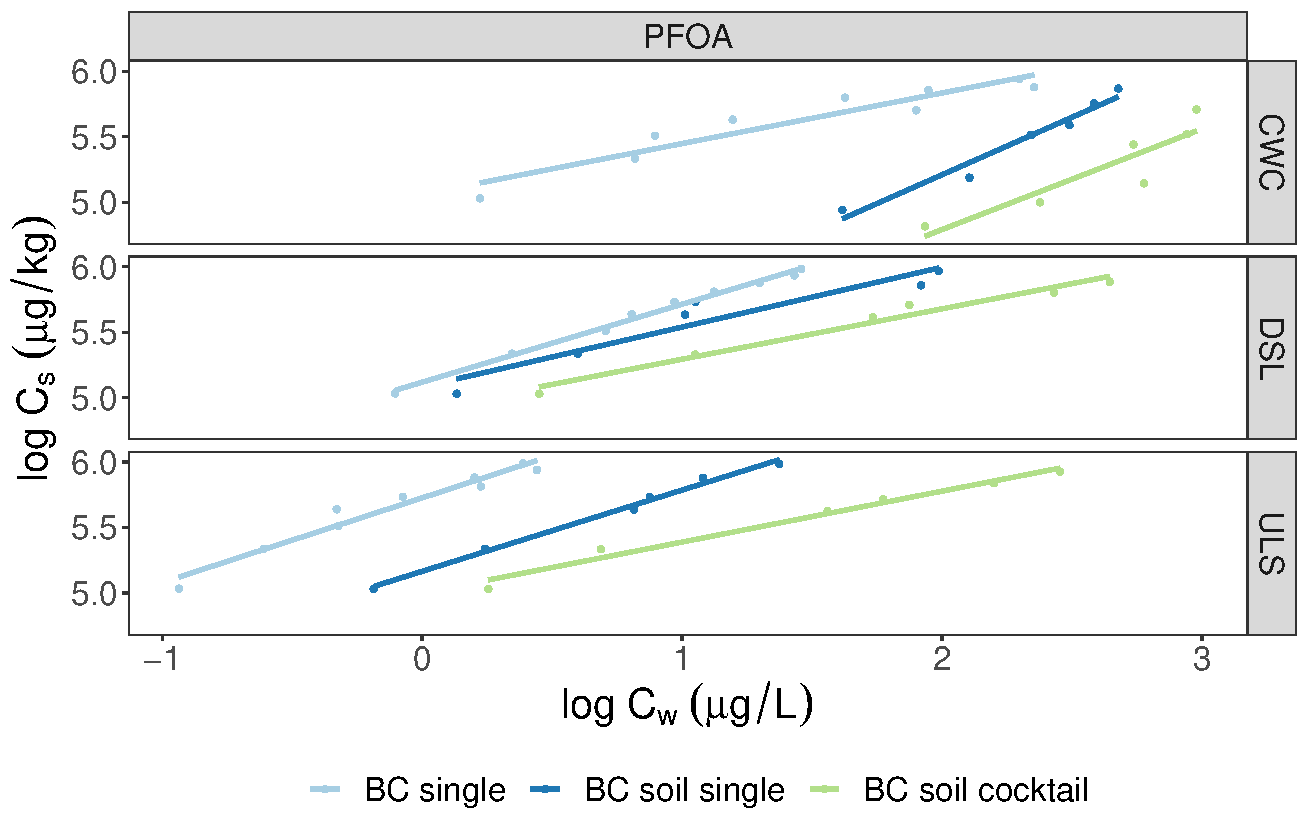
\includegraphics[width=\textwidth]{R/figs/Attenuation_isotherms_PFOA.pdf}
    \caption{Sorption isotherm comparison for PFOA single-compound spike in biochar (BC single), single-compound spike in soil-biochar (BC soil single), and PFOA spiked in a cocktail in soil-biochar showing attenuation by soil and competing congeners.}
    \label{fig:PFOA_attenuation}
\end{figure}

\subsection{Freundlich sorption non-linearity}\label{sec:non-linearity}
The non-linear sorption isotherms for PFOA in \cref{fig:PFOA_nonlinear} show how sorption is attenuated at higher concentrations, and how attenuation changes in the presence of soil and soil with other PFCAs. The resulting Freundlich coefficients ($\log~K_F$ and $n_F$) for PFOA are given in \cref{tab:PFOA_Freundlich}, and the remaining compounds are in \cref{appSec:Sorption}\cref{apptab:summary_stats_all}. Two general conclusions can be drawn from these figures: 1) attenuation is higher in the presence of soil, and even higher when soil and cocktail are added together. And 2) the concentration intervals for some of the isotherms were too narrow (average $\Delta~\log~C_w$ = 1.3) to properly determine representative Freundlich coefficients for a wider concentration range. Therefore, conversion of $\log~K_F$ to either higher or lower units can be expected to be associated with greater uncertainty.

Both concentration intervals and $n_F$ should be considered together in order to predict the sorption capacity of biochars. \Cref{fig:nonlinear_OND} shows the non-linear BC-single isotherms for PFOA, PFNA and PFDA, where the degree of non-linearity is more easily visualized than the $n_F$-values alone. For example, \cref{fig:nonlinear_OND} shows that the CWC biochar isotherms have more attenuation than DSL and ULS biochars, and that $C_w$s have measurements across a wider concentration range. These findings are consistent with lower $\log~K_F$s found for CWC. \cref{fig:nonlinear_OND} also shows that the isotherms for PFNA-DSL and PFNA-ULS are nearly linear, and span aqueous concentrations only within the same order of magnitude. Higher spike concentrations, or lower BC dosages, should have been used to get isotherms that cover the regions of attenuated sorption for these biochars and compounds. What is significant is that this suggests that sludge biochars have higher sorption capacities than CWC.

The concentration range achieved for $C_w$ for the sorption isotherms was an average of 1.3 $\log$ units, in contrast to the desired concentration range over 4 $\log$ units. Poor signals were achieved for the SC1 points, and as a result were removed from the data analysis. This resulted in the spike concentration interval being reduced to two orders of magnitude (\cref{tab:spikeConcentrations}). In retrospect, spike concentrations at each $\log$ unit should have been selected instead of spreading the ten concentrations evenly across the concentration range. The CWC isotherms had the widest concentration intervals for $C_w$. This can be accounted for by the fact that CWC is the weakest sorbent of the three biochars studied.  

Electrostatic interactions between PFCAs and sediment can contribute to enhancing saturation of adsorption sites as well as intermolecular electrostatic repulsion between individual molecules \citep{higgins2006sorption,yin2022insights}. \cite{yin2022insights} presents two main explanations for why sorption of PFCAs to biochar is non-linear: 1) successive saturation of adsorption sites, and 2) the complex composition of biochar with negative, positive and neutral charges within same matrix. 

\begin{table}
\caption{Freundlich distribution coefficients and standard errors for the PFOA isotherms. Freundlich coefficients for the soil samples are the collective partition coefficients for soil and biochar because $K_d$ for soil alone was not accurate enough. All $K_F$ data are in units of $\mathrm{(\mu g/kg)/(\mu g/L)^{n_F}}$.}
\centering
\adjustbox{max width=\textwidth}{%
\begin{threeparttable}
\label{tab:PFOA_Freundlich}
\begin{tabular}{lllllll} \toprule
\multicolumn{1}{c}{Compound} & \multicolumn{1}{c}{Biochar} & \multicolumn{1}{c}{type} & \multicolumn{1}{c}{$\log~K_F$} & \multicolumn{1}{c}{$n_F$} & \multicolumn{1}{c}{$r^2$} & \multicolumn{1}{c}{$p$} \\ \midrule
PFOA & CWC & BC-S-mix  & 3.25 ± 0.48 & 0.77 ± 0.18 & 0.82 & * \\
PFOA & CWC & BC-S-sing & 3.45 ± 0.21 & 0.88 ± 0.09 & 0.96 & ** \\
PFOA & CWC & BC-sing    & 5.06 ± 0.08 & 0.39 ± 0.05 & 0.90 & *** \\
PFOA & DSL & BC-S-mix  & 4.91 ± 0.06 & 0.39 ± 0.03 & 0.97 & *** \\
PFOA & DSL & BC-S-sing & 5.08 ± 0.10 & 0.46 ± 0.08 & 0.90 & * \\
PFOA & DSL & BC-sing    & 5.12 ± 0.02 & 0.60 ± 0.02 & 0.99 & *** \\
PFOA & ULS & BC-S-mix  & 5.00 ± 0.05 & 0.39 ± 0.03 & 0.98 & *** \\
PFOA & ULS & BC-S-sing & 5.16 ± 0.03 & 0.62 ± 0.03 & 0.99 & *** \\
PFOA & ULS & BC-sing    & 5.73 ± 0.02 & 0.65 ± 0.05 & 0.95 & *** \\ \bottomrule
\end{tabular}
\begin{tablenotes}
\item Significant codes: *** $\sim$ 0.001, ** $\sim$ 0.01, * $\sim$ 0.05
\end{tablenotes}
\end{threeparttable}}
\end{table}

\begin{figure}
    \centering
    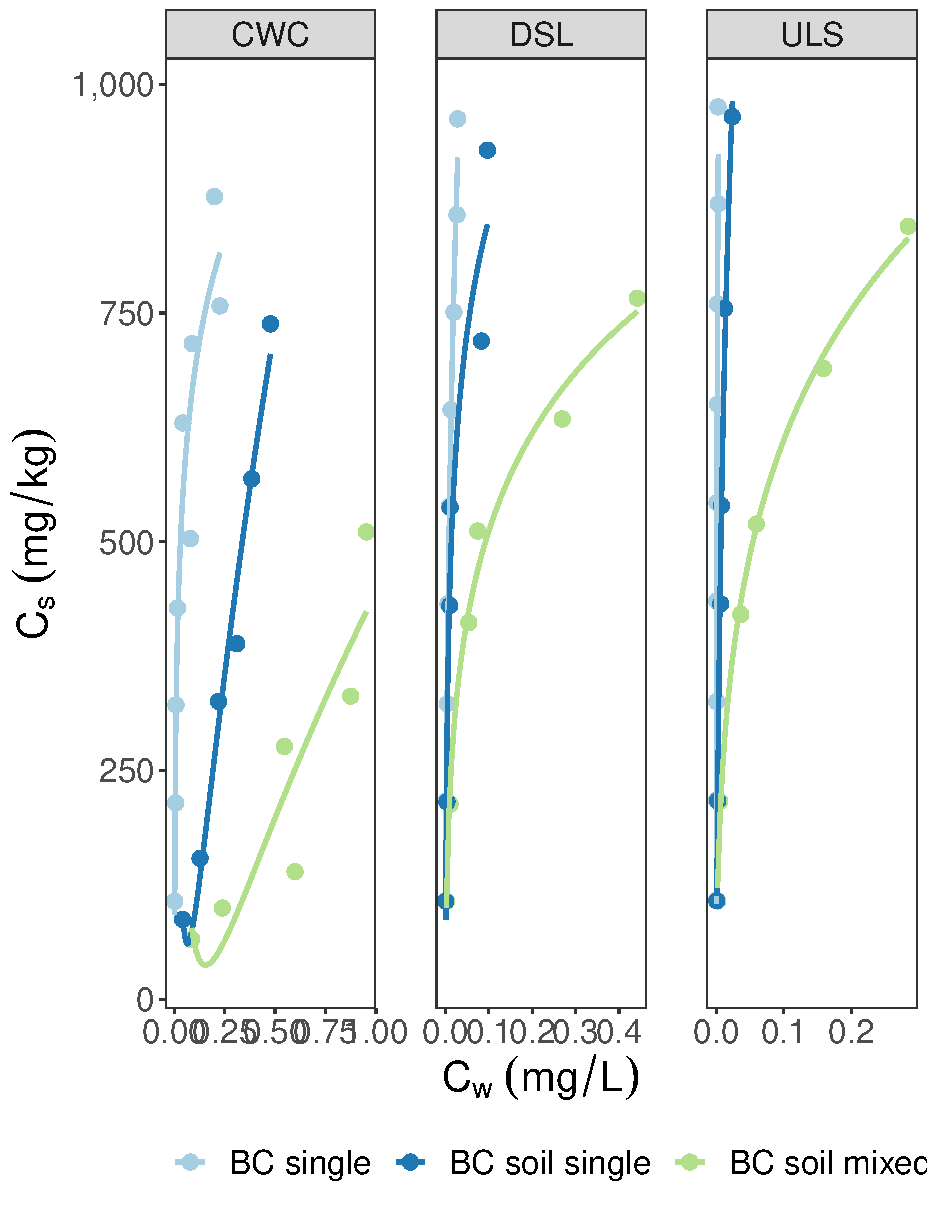
\includegraphics[width=\textwidth]{R/figs/PFOA_linear.pdf}
    \caption{Non-linear sorption isotherms for PFOA in the BC-single, BC-mixed and BC-soil-mixed batch tests. Lines are fitted by a polylogarithmic function.}
    \label{fig:PFOA_nonlinear}
\end{figure}

\begin{figure}
    \centering
    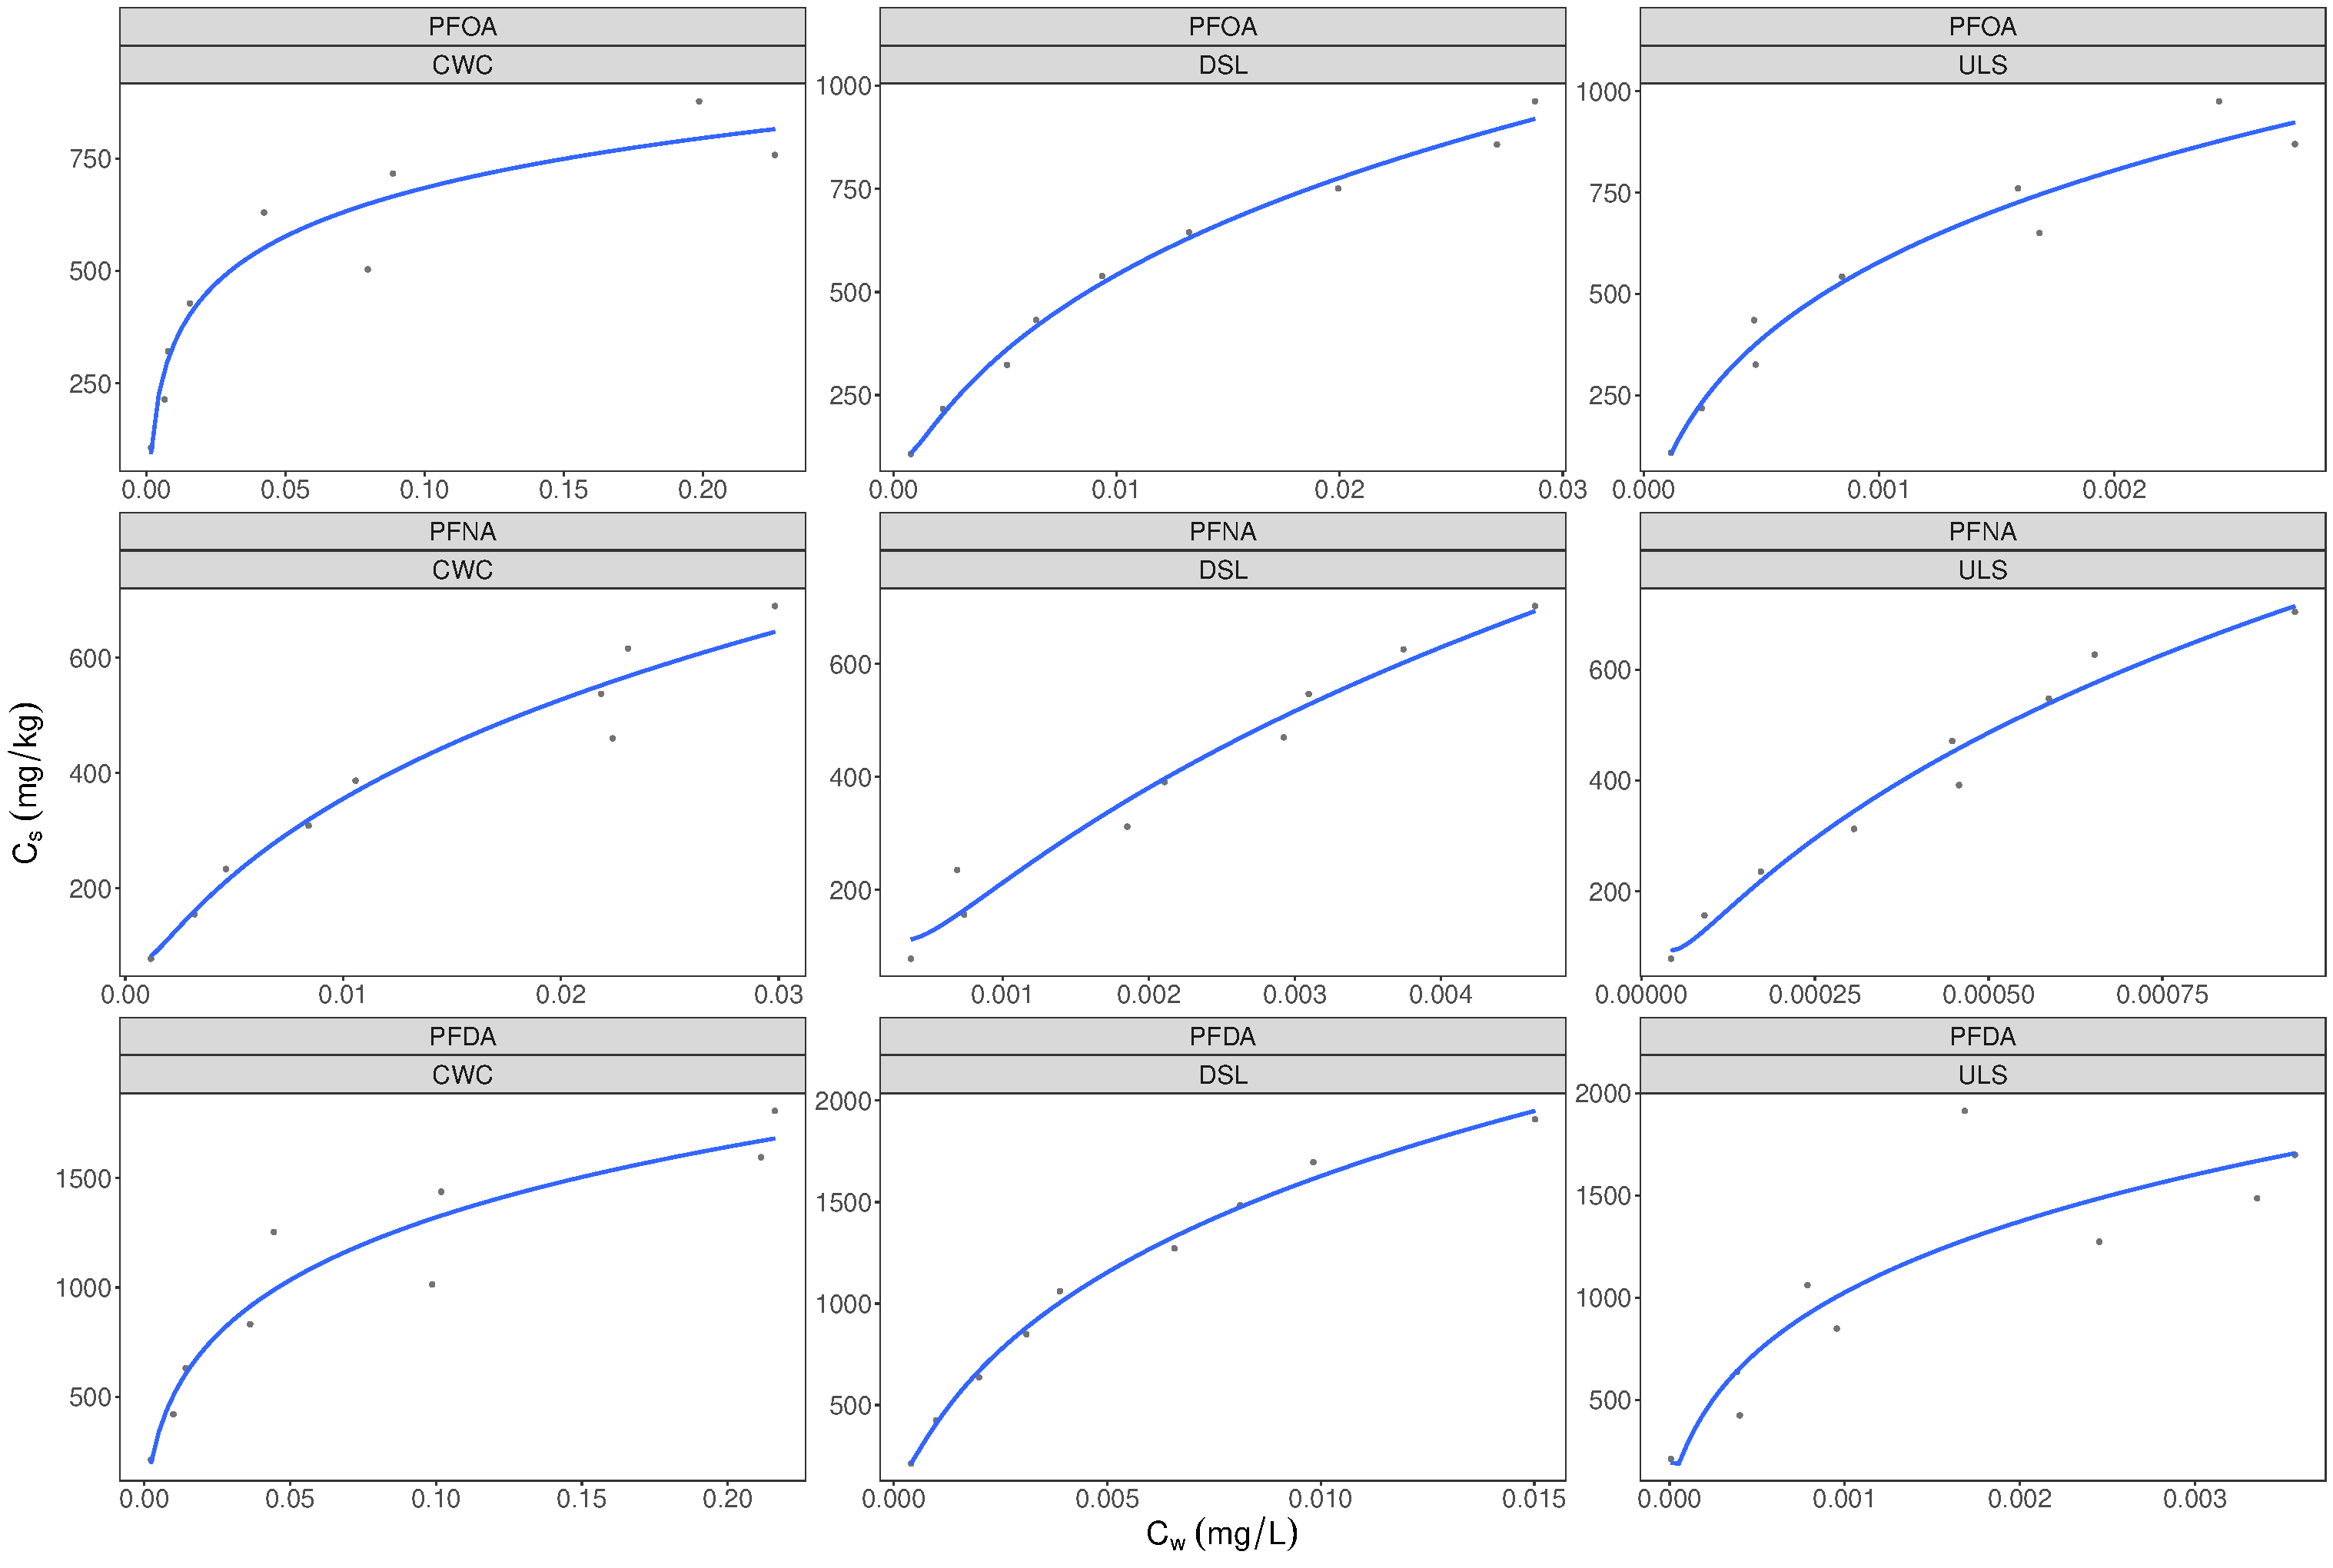
\includegraphics[width=\textwidth]{R/figs/BC_single_attenuation.pdf}
    \caption{Plots showing sorption attenuation by the presence of other PFCAs with increasing spiked concentrations. Lines are fitted by a polylogarithmic function.}
    \label{fig:nonlinear_OND} 
\end{figure}

\subsection{Attenuation by organic matter} 
Colored filtrate and humus aggregation seen during analysis of the soil batch tests indicate that sorption of organic matter (OM) to biochar is likely (see \cref{sec:batch}. Large humic acids (300-600 nm) clog the pores, preventing diffusion of PFAS \citep{Cornelissen2006,kluvcakova2018size}. Furthermore, the size of the organic molecules is a critical factor, as humic molecules, whose size is similar to that of PFAS, represent the greatest competition to PFAS in terms of diffusion \citep{du2014adsorption}. By the co-existence of OM and dissolved organic carbon (\acrshort{DOC}), sorption attenuation occurs by a combination of competitive and weaker sorption of PFAS to OM and DOC, and the competitive sorption of OM to biochar. PFAS binds to OM, and it is possible that PFAS also binds to the dissolved fraction of OM (DOC). Since DOC is sorbed it is thus possible that there is sorption of DOC-PFAS complexes. Given that DOC-assisted PFAS sorption has yet not been proven, and investigating size fractionation for humic molecules was not a part of this study, the points presented here could only take place on a theoretical level.




